% auteur template : Christophe Adam
% template réalisé pour les TFE de la HEPL afin de 
%  faciliter la rédaction et la mise en page.

% Ressource intéressante pour LateX et le TFE : https://www.youtube.com/watch?v=zqQM66uAig0

% !TeX encoding = UTF−8
% !TeX program = pdflatex
% !TeX spellcheck = fr_FR
\documentclass[a4paper,12pt]{report}
%% Partie packages et mise en page
\usepackage{graphicx}
\usepackage{pifont}
\usepackage[T1]{fontenc}
\usepackage[french]{babel} % si vous rédigez en anglais, il sera nécessaire d'update les packages de langue
\usepackage{lmodern}
\usepackage[autolanguage]{numprint} % for the \nombre command
\usepackage[margin=25mm, includeheadfoot, bindingoffset=6mm]{geometry}
\usepackage{fancyhdr}
\usepackage{xcolor}
\usepackage{amsmath}
\usepackage{blindtext}
\usepackage{float}
\usepackage{wrapfig}
\usepackage{pdfpages}
\usepackage{url}
\usepackage{hyperref}
\usepackage{listings}
\usepackage{subcaption}
\usepackage{titlesec}
\usepackage{enumitem}
\renewcommand{\thesubsubsection}{\arabic{subsubsection}. }


\usepackage[skip=15pt plus1pt, indent=5pt]{parskip}
\graphicspath{{images/}}

% Partie pour créer des bouts de codes dans le document
\definecolor{codegreen}{rgb}{0,0.6,0}
\definecolor{codegray}{rgb}{0.5,0.5,0.5}
\definecolor{codepurple}{rgb}{0.58,0,0.82}
\definecolor{backcolour}{rgb}{0.95,0.95,0.93}
\lstdefinestyle{mystyle}{
    backgroundcolor=\color{backcolour},   
    commentstyle=\color{codegreen},
    keywordstyle=\color{magenta},
    numberstyle=\tiny\color{codegray},
    stringstyle=\color{codepurple},
    basicstyle=\ttfamily\footnotesize,
    breakatwhitespace=false,         
    breaklines=true,                 
    captionpos=b,                    
    keepspaces=true,                 
    numbers=left,                    
    numbersep=5pt,                  
    showspaces=false,                
    showstringspaces=false,
    showtabs=false,                  
    tabsize=2
}
\lstset{style=mystyle}

% Fancy permet la mise en page avec le chapitre en haut à droite ainsi que d'autres paramètres
\pagestyle{fancy}
\fancyhead{}
\fancyhead[R]{Chapitre \thechapter}
\fancyhead[L]{\nouppercase{\rightmark}}
\fancyfoot{}
\fancyfoot[C]{\thepage}
\fancyfoot[L]{\nouppercase{Molka ABID}}
\renewcommand{\headrulewidth}{0.3pt}
\renewcommand{\footrulewidth}{0pt}

\setlength{\headheight}{15pt}
\linespread{1.5}
\counterwithin{figure}{section}


% Début du document en lui-même

\begin{document}
% À changer avec la bonne page de garde de l'école
 \includepdf[pages=1]{page de garde/page.pdf}

% Beginning
\chapter*{Remerciements}

   At this critical point in my career and training, I must take a minute to convey my thanks to everyone who has contributed to my experience at SOMFY, particularly at the SOMFY ZRIBA industrial site. This internship with this firm, the world leader in motion automation for home and building, has been an enriching and transformational experience thanks to the kind supervision of my supervisors.
First and foremost, I'd like to thank Maxime LORIN, Digital Engineering Manager, and Ludwig Taubert, full stack developer, for their great assistance and experience.
I also like to thank Khaled ABDELWAHER, the laboratory's manager, for his leadership and direction. Their advice and assistance have been invaluable to my professional progress, and I am really thankful for this chance.
I would also want to thank the whole SOMFY ZRIBA maintenance crew. The colleagues I had the pleasure of working with greeted me with compassion and professionalism, making the experience even more enjoyable.
Finally, I'd want to thank SOMFY ZRIBA's management for the opportunity to join a worldwide famous firm and contribute to its projects.
Overall, I would want to express my heartfelt gratitude to everyone who contributed in any manner to this pivotal and formative experience at SOMFY ZRIBA.


\chapter*{Abstract}
As part of Industry 4.0, digital transformation of industrial processes is critical for increasing operational efficiency, flexibility, and sustainability. This approach uses modern technologies like the Internet of Things (IoT) and data analytics to build intelligent, networked manufacturing systems. This method is consistent with the United Nations' Sustainable Development Goal 9 (SDG 9), which aims to strengthen infrastructure, promote equitable and sustainable industrialization, and encourage innovation.The LAB.E.S project is entirely aligned with this dynamic, as it creates an innovative platform for real-time monitoring of laboratory operations. Although we did not work directly with artificial intelligence, our primary responsibility was to remove all paperwork in the lab and digitize all operations.


\vspace{2cm}




\chapter*{Disclaimer}
We regret to readers for the likely presence of French words in some of the diagrams, photos, and appendices in this research project. There are various explanations for this. To begin, the project's parent corporation is situated in France, and the early development team was primarily composed of French-speaking members. Second, while the project was intended to be worldwide in scope and implemented in all of the company's laboratories throughout the world, certain documents and graphics were created in a framework where French was the primary working language. Finally, changes in the development team throughout the course of the project resulted in contributions from a variety of persons, perhaps adding to the linguistic diversity.
While every attempt has been taken to unify material and guarantee general consistency, some graphic sections or appendices may nevertheless include French. We trust that these differences do not impede your general comprehension or the aim of this report, and we thank you in advance for your patience and understanding.


\vspace{2cm}


% Tables matières et figures
\tableofcontents
\listoffigures

% Part 1
\part{Introduction et Background}


% Chapitres

\chapter{ State of art \\
Internet Industriel des Objets (IIoT)}
\section{Introduction}
The IoT has disrupted numerous industries by making devices secure, intelligent and connected; it enables process optimization and provides data-driven decision making. For my first foray into the Internet of Things, I learned fundamental skills for designing and integrating connected systems. From this experience I was then able to progress onto a higher level, that of the IIoT (Industrial Internet of Things) where I could take my initial learnings, and focus them towards more complex industrial application-focussed environments.
\begin{figure}[H]
    \centering
    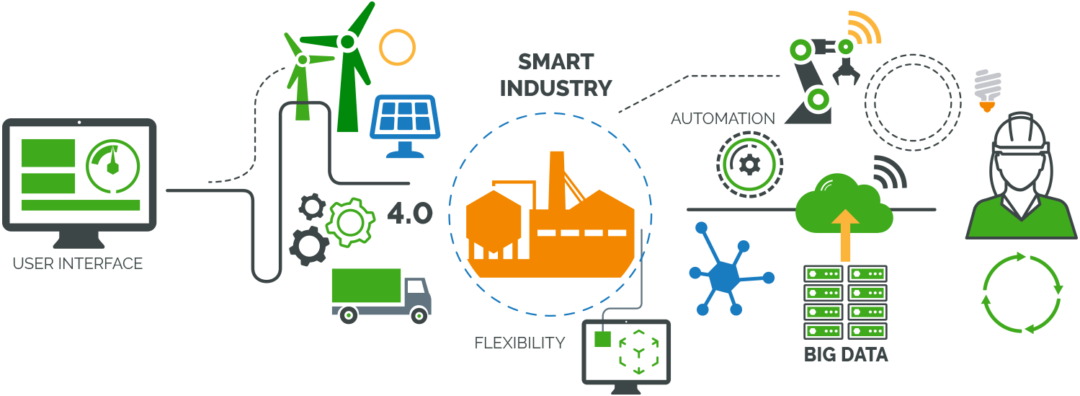
\includegraphics[width=0.7\textwidth]{chapters/N-1/img/what-is-industrial-Internet-of-things-1080x396.png}
    \caption{Somfy Zriba Products}
    \label{fig:campus}
\end{figure}

\section{L’IoT et l’IIoT}
While the principles behind IoT and IIoT are similar, their requirements are different. IoT is mostly aimed at consumers, whereas IIoT is for industrial setups such as manufacturing, energy and infrastructure. In my case, this transition from IoT to IIoT was important because now I am trying to solve some technical challenges like system resilient, more secure and real-time data handling.

\section{Les architectures de référence}
Robust reference architectures are the foundation upon which IIoT operates, and they are created to ensure seamless interoperability, securing system scale. These models can be one of the three-tier architecture (perception, network and application) model which provide a systematic way to govern data stream from sensors up-to analysis and visualization platform. These principles are utilized in this project, where secure gateways relay data from industrial sensors to advanced processing systems.

\section{Qualité de service dans l'IIoT}
Quality of Service (QoS) is an essential aspect in IIoT systems that ensures performance, dependability and confidentiality communications. In an industrial environment, a minor failure or delay results in significant losses. As part of my IIoT exposure I had to pay close attention to various QoS mechanisms, specially for realtime monitoring of industrial equipment that needs immediate and timely transfer of data.
\chapter{Présentation Génerale}

Picture a busy lab where everything is operating effectively and without hiccups. The Laboratory Execution System (LAB.E.S) project was created with that goal in mind. LAB.E.S is poised to revolutionize lab operations by offering a state-of-the-art platform that centralizes data with ease and monitors activity in real-time.
LAB.E.S offers an all-inclusive solution to optimize laboratory procedures by combining the most recent technological developments with an emphasis on the users. As a result, the lab's work is not only quicker but also more dependable due to increased production and superior test findings.
\section{Description de l'entreprise}

One prominent participant in the industrial automation sector is Somfy Zriba, a proud affiliate of the SOMFY Group. Its specialty is the design and production of necessary machinery for movement automation, with a focus on closures and sun protection. Somfy Zriba exemplifies SOMFY's dedication to automation excellence while building on its heritage and reputation.
Somfy Zriba has changed dramatically since its founding, going from trailblazer to unchallenged leader. This development has been made possible by a persistent dedication to sustainability, innovation, and quality. Over the years, Somfy Zriba has adhered to SOMFY's mission to create safer, more environmentally conscious, and more livable houses and structures.
\begin{figure}[H]
    \centering
    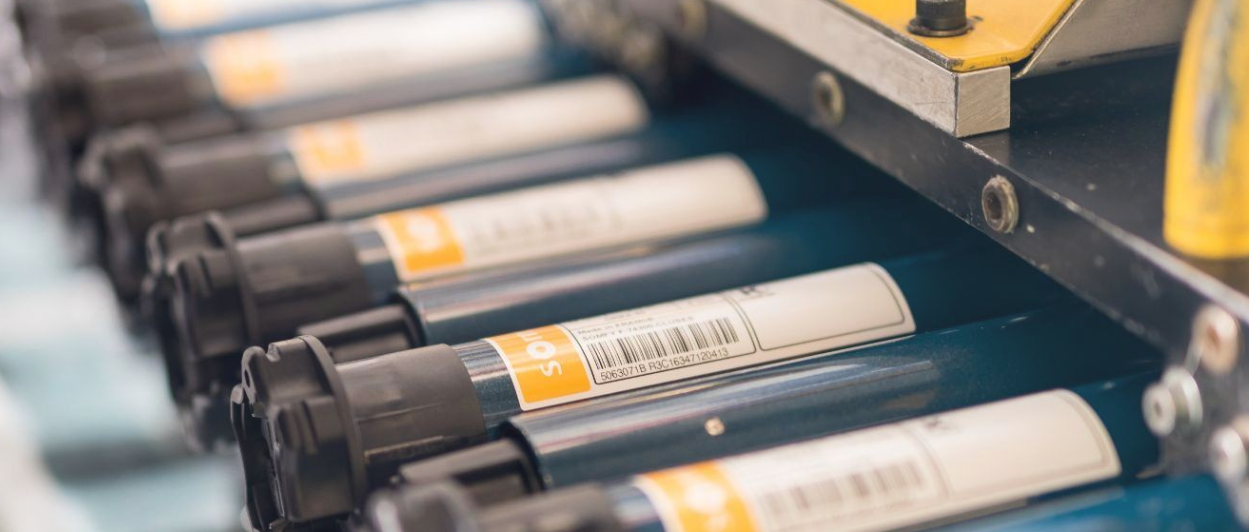
\includegraphics[width=1\textwidth]{chapters/1/img/sitemmoto.png}
    \caption{Somfy Zriba Products}
    \label{fig:campus}
\end{figure}
Somfy Zriba's business encompasses the design and production of automated devices such as motors and controls. These components play an essential role in facilitating the daily lives of users around the world. 

\section{La strategie en action}
\begin{enumerate}
	\item Using Automated Techniques to Enhance Building Energy Performance: Put automated solutions into place to maximize building energy use and promote environmental sustainability.
	\item  Act for Green®: The Group's Strategy for Eco-Friendly Product Design To lessen the environmental impact and encourage eco-friendly behaviors, concentrate on developing sustainable products.
    \item  Improving the Customer Experience with Digitalization: Make sure that all group customers have access to the TaHoma® linked home ecosystem and enhance customer interactions by utilizing digital tools.
    \item “Building Together" with Suppliers: To ensure shared success and innovation, fortify partnerships with suppliers to promote a collaborative approach.
    \item Encouraging and Involving Workers to Increase the Group's Influence: Promote employee engagement and motivation to support the group's mission, which will have a favorable and significant effect on the market.
\end{enumerate}








\section{Description de l'Environnement de Travail}

In order to promote innovation and ongoing development, our organization places a high value on its ENGINEERING{\&}CUSTOMER SATISFACTION department, formerly known as Research and Development (R{\&}D). Numerous strategic efforts aimed at enhancing strategic alignment, encouraging project management autonomy, maximizing operational efficiency, and supporting the industrialization process are examples of its dedication.

The dedication of the Engineering & Customer Satisfaction department is shown by:
\begin{itemize}[label=\textbullet, font=\LARGE]
    \item Supporting sustained technical excellence, procedures, and technological infrastructures in order to increase SOMFY's potential for innovation.
    \item Creating and producing Somfy goods and services in compliance with the necessary requirements.
    \item Establish an outstanding IT infrastructure to aid in our company's digital transformation.
\end{itemize}



\section{Cadre général du projet}


Through the introduction of a platform for data consolidation and real-time monitoring, the Laboratoire Execution System (LAB.E.S) seeks to revolutionize laboratory administration.
To evaluate the effects on workflow and test result quality, a comparison study between traditional laboratory work practices and the digitalization of the profession was conducted within this framework.
One of the most important steps toward increasing operational effectiveness and test result quality is the digitalization of laboratory operations. The modernization of laboratory management procedures is the foundation of this project, which attests to the shift to more effective and scalable procedures.
\begin{figure}[H]
    \centering
    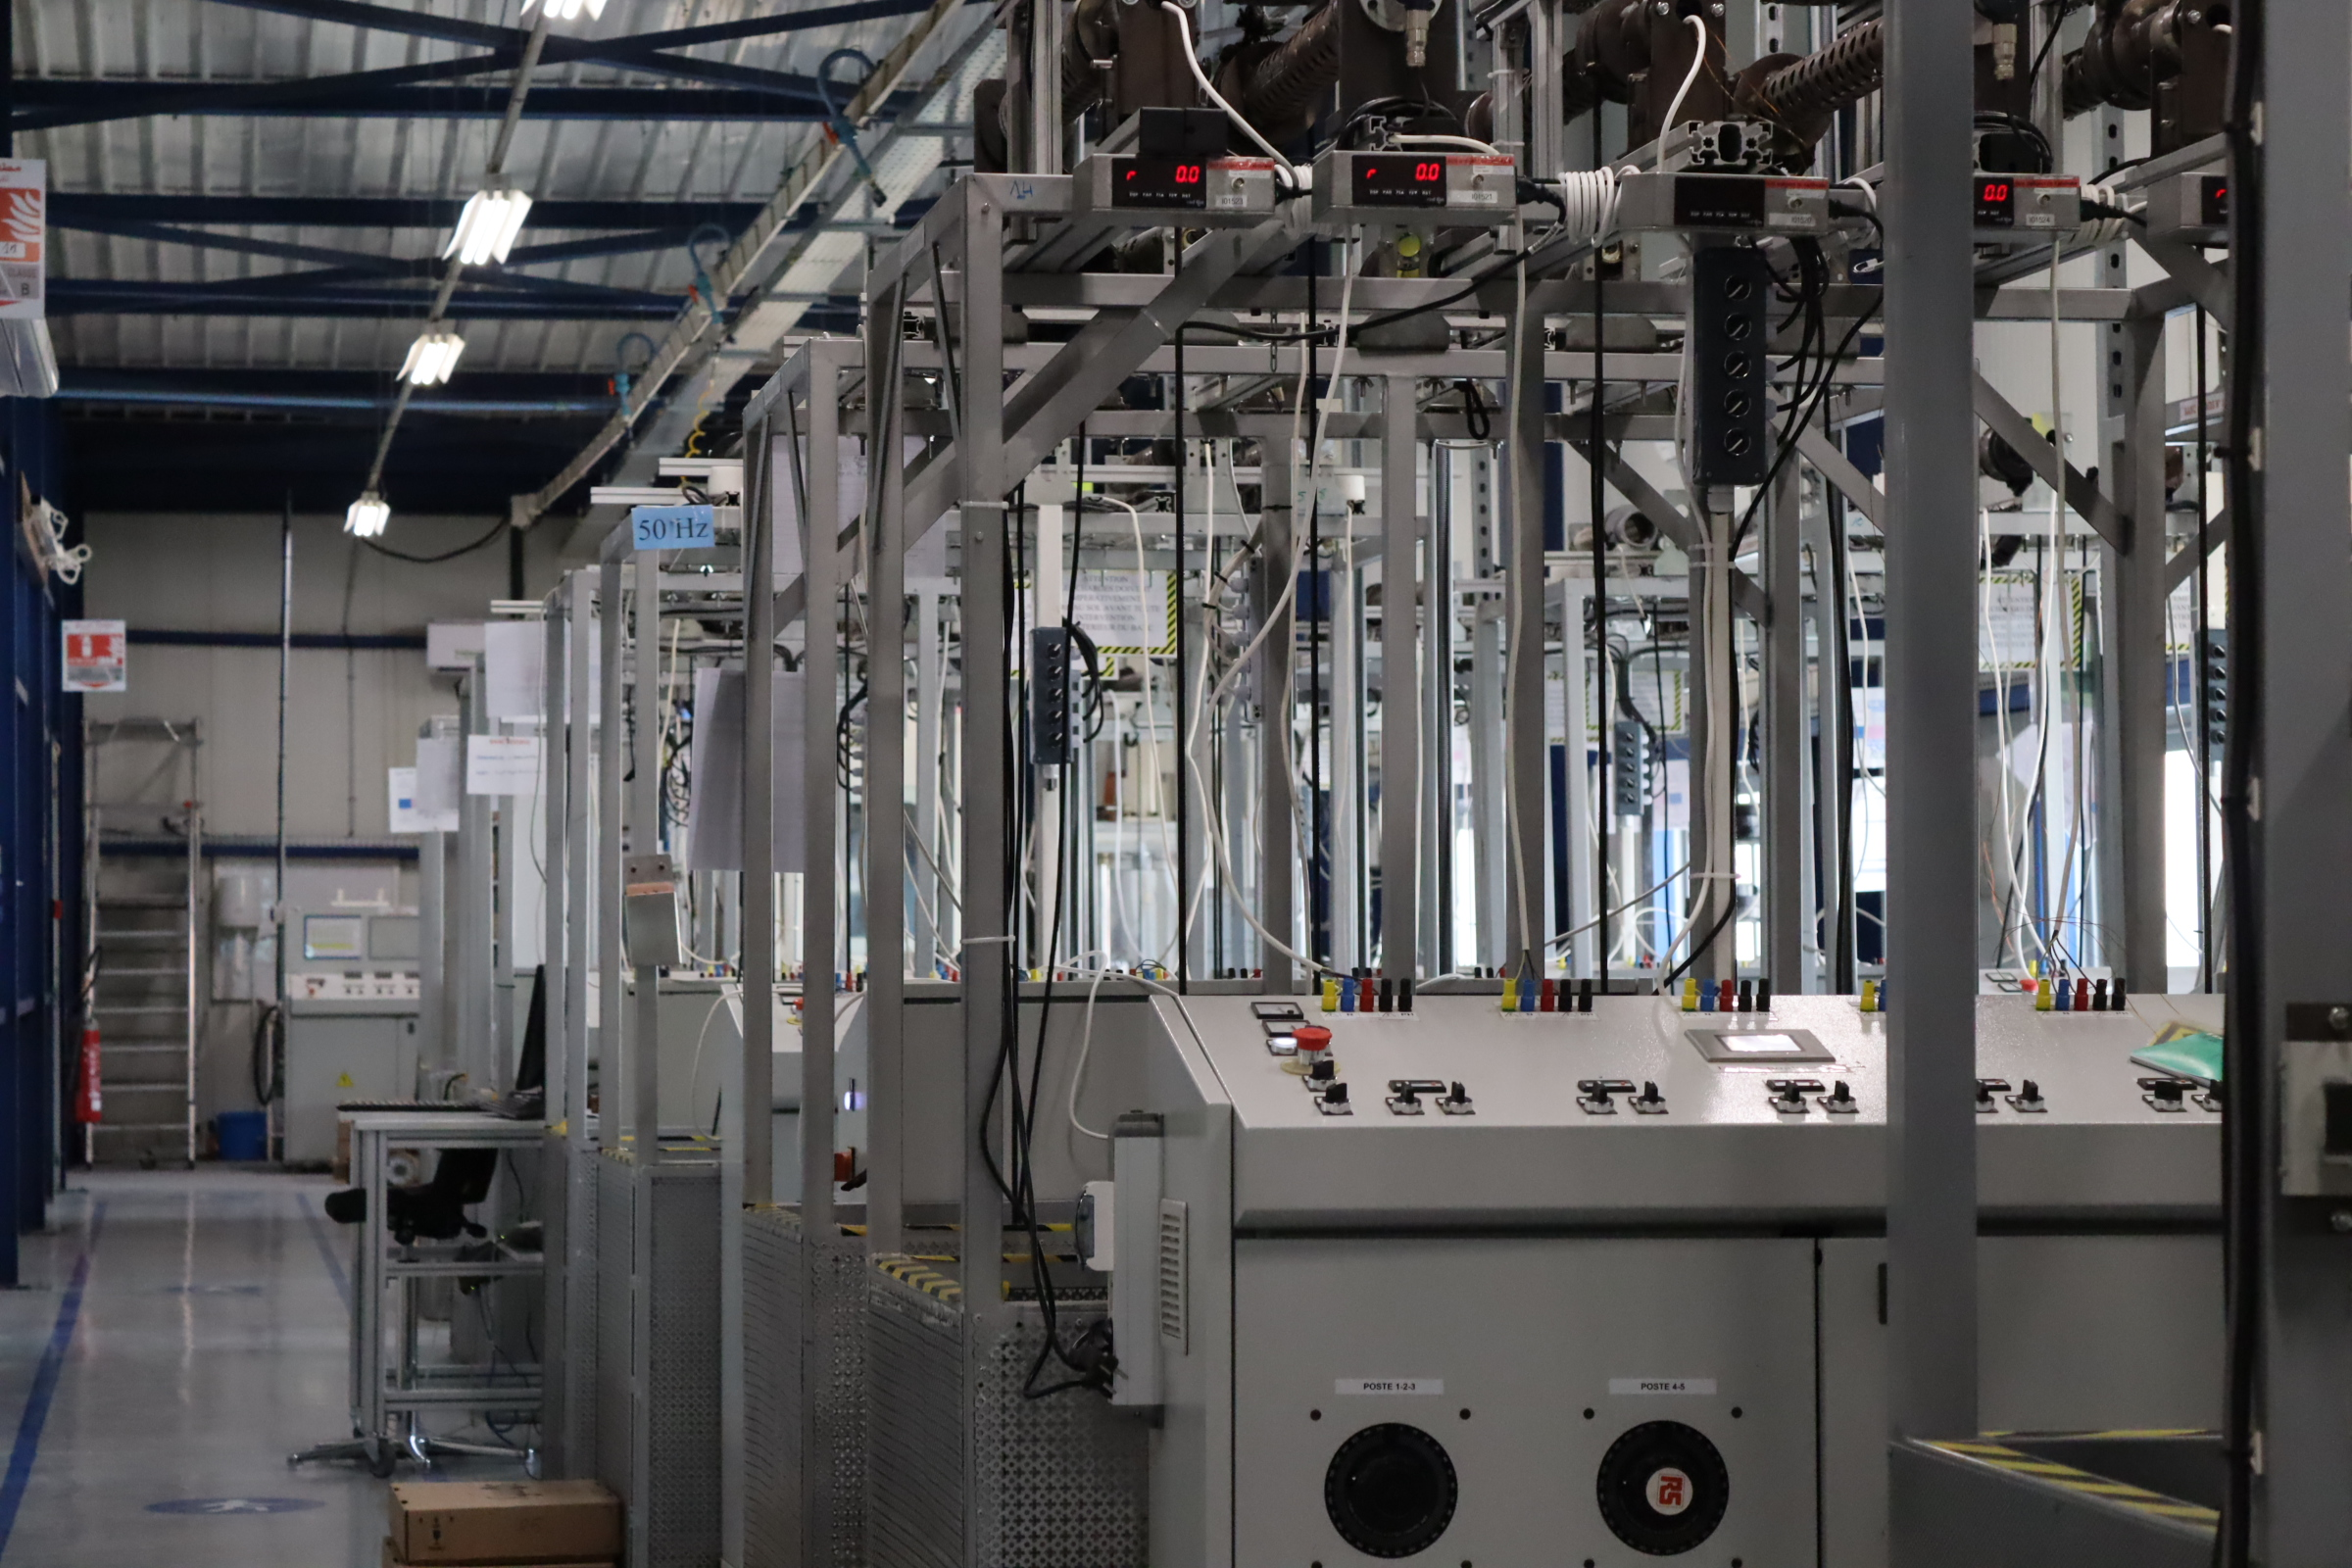
\includegraphics[width=1\textwidth]{chapters/1/img/IMG_0258.JPG}
    \caption{Somfy Zriba Lab}
    \label{fig:campus}
\end{figure}
The journey of this ambitious endeavor is detailed in this report, which highlights significant turning points, difficulties faced, and solutions put in place to change the scene of laboratory operations. 
We have created a design for the deployment of a strong and creative system that is equipped to handle the problems of the contemporary world by investigating cutting-edge technology and modifying industry best practices.
In these pages, we examine the differences and similarities between typical laboratory work and work carried out with LAB.E.S. We look at how it affects productivity, workflow, and test result quality. We will demonstrate the strategic significance of this change for laboratory operations in the future by examining the observable advantages and measurable gains.
Our dedication to quality and our common goal of innovation in laboratory management are evident in this report. It provides a useful viewpoint on both the prospects presented by the digitalization of labor and the difficulties we encounter in achieving this goal in a dynamic industrial setting.










\section{Aproche de travail}
After introducing the company and defining the scope of the project, it is critical to describe the working strategy used to bring this project to completion. We picked the Scrum technique, which is an agile approach to complicated project management designed to promote flexibility, cooperation, and efficiency. This chapter teaches Scrum concepts, team responsibilities, and how to plan and monitor project progress using a Gantt chart.

\subsection{Principe de Scrum}
Scrum is an agile project management methodology that uses iterative and incremental approaches. The primary characteristics of Scrum are:

\begin{enumerate}
  \item Sprints: Work iterations that extend from two to four weeks in which we build and deliver an element of the product.
  \item Increment: At the end of each sprint, a functional increment that adds value is delivered. 
  \item Regular meetings: In addition to sprint planning meetings, sprint reviews, and retrospectives, I collaborate weekly with Mr Ludwig Taeubert, Full Stack Developer, who offers technical guidance. These meetings allow me to track the status of assignments, fix technological issues and improve coordination.
 
\end{enumerate}




\subsection{Rôles dans une Équipe Scrum}
To manage the project, we used the Scrum agile methodology, which allows for an iterative, incremental approach. This technique is founded on a number of important ideas and responsibilities that have guided our development team.
\begin{description}
  \item[Product Owner (PO):] Mr Khaled Abdelwaheb, Plant Laboratory Manager. He is responsible for defining product requirements and managing the backlog. His role is to ensure that business needs are correctly translated into functionalities.
  \item[Scrum Master:] Mr Maxime Loren, Digital Engineering Manager. He facilitates the Scrum process, supports the team in removing obstacles and ensures the application of agile best practices.
  \item[Development team:] The development team, of which I am the sole member, is in charge of providing functional increments each sprint. We are in charge of technological implementation and job fulfillment in accordance with the sprint backlog.
\end{description}


\subsection{Utilisation du Diagramme de Gantt}
Although Scrum focuses on iterative development and adaptability, we also used a Gantt chart to plan and monitor the project's key stages. The tool gave a detailed picture of projects, deadlines, and dependencies, allowing the team to coordinate more effectively. The Gantt chart for our project was organized as follows:

\begin{enumerate}
  \item Phase Definition: The project was divided into four primary phases: initial planning, development, testing, and release. These phases have been clearly outlined to help advancement.
  \item Tasks and Subtasks: Each phase was divided into distinct tasks and subtasks that were explicitly assigned to members of the development team. This made it easier to assign roles and track individual efforts.
  \item Tracking Deadlines and Progress: The Gantt chart was used to monitor the progress of the individual activities, detect any delays, and alter priorities as needed to ensure that the overall project deadlines were reached.
  \item Dependency Management: Task dependencies, such as the one between requirements collecting and finalization, were clearly specified. This allowed for more proactive risk management and interdependence among project stages.
\end{enumerate}




% Part 2
\part{Etude de cas}
\chapter{Analyse des Besoins et Identification des Utilisateurs}

To comprehend the internal dynamics and difficulties the laboratory encounters, a thorough examination of its current circumstances and environment is essential. This chapter's objective is to give a summary of the laboratory's current operating procedures, technological advancements, and organizational structure. Finding processes' advantages, disadvantages, and potential for improvement and modernization is the goal.
We'll start by examining the laboratory's structure and organization, emphasizing the functions and duties of the different participants. We'll then examine the difficulties with the present procedure, including operational flaws and technology limitations. To increase the laboratory's overall effectiveness and performance, we will examine current technology solutions and investigate possibilities of further technological advancement.

\clearpage
\section{ Structure et Organisation du Laboratoire}


\subsection{Fonctionnement du Laboratoire}


\subsection{Probléme et Defis du Fonctionnement du Laboratoire}

The Somfy laboratory functions independently of the company's industrial operations. During an in-depth investigation of its operation, a fundamental issue was discovered: the work process is not digital, resulting in a lack of consistency between laboratory test data, test sheets, and test results. This lack of digital integration can cause inefficiencies and gaps in data management, thus affecting the quality and traceability of the tests performed.


\subsection{Intégration du Digital dans les Systèmes de Fonctionnement du Laboratoire}

\begin{figure}[H]
    \centering
    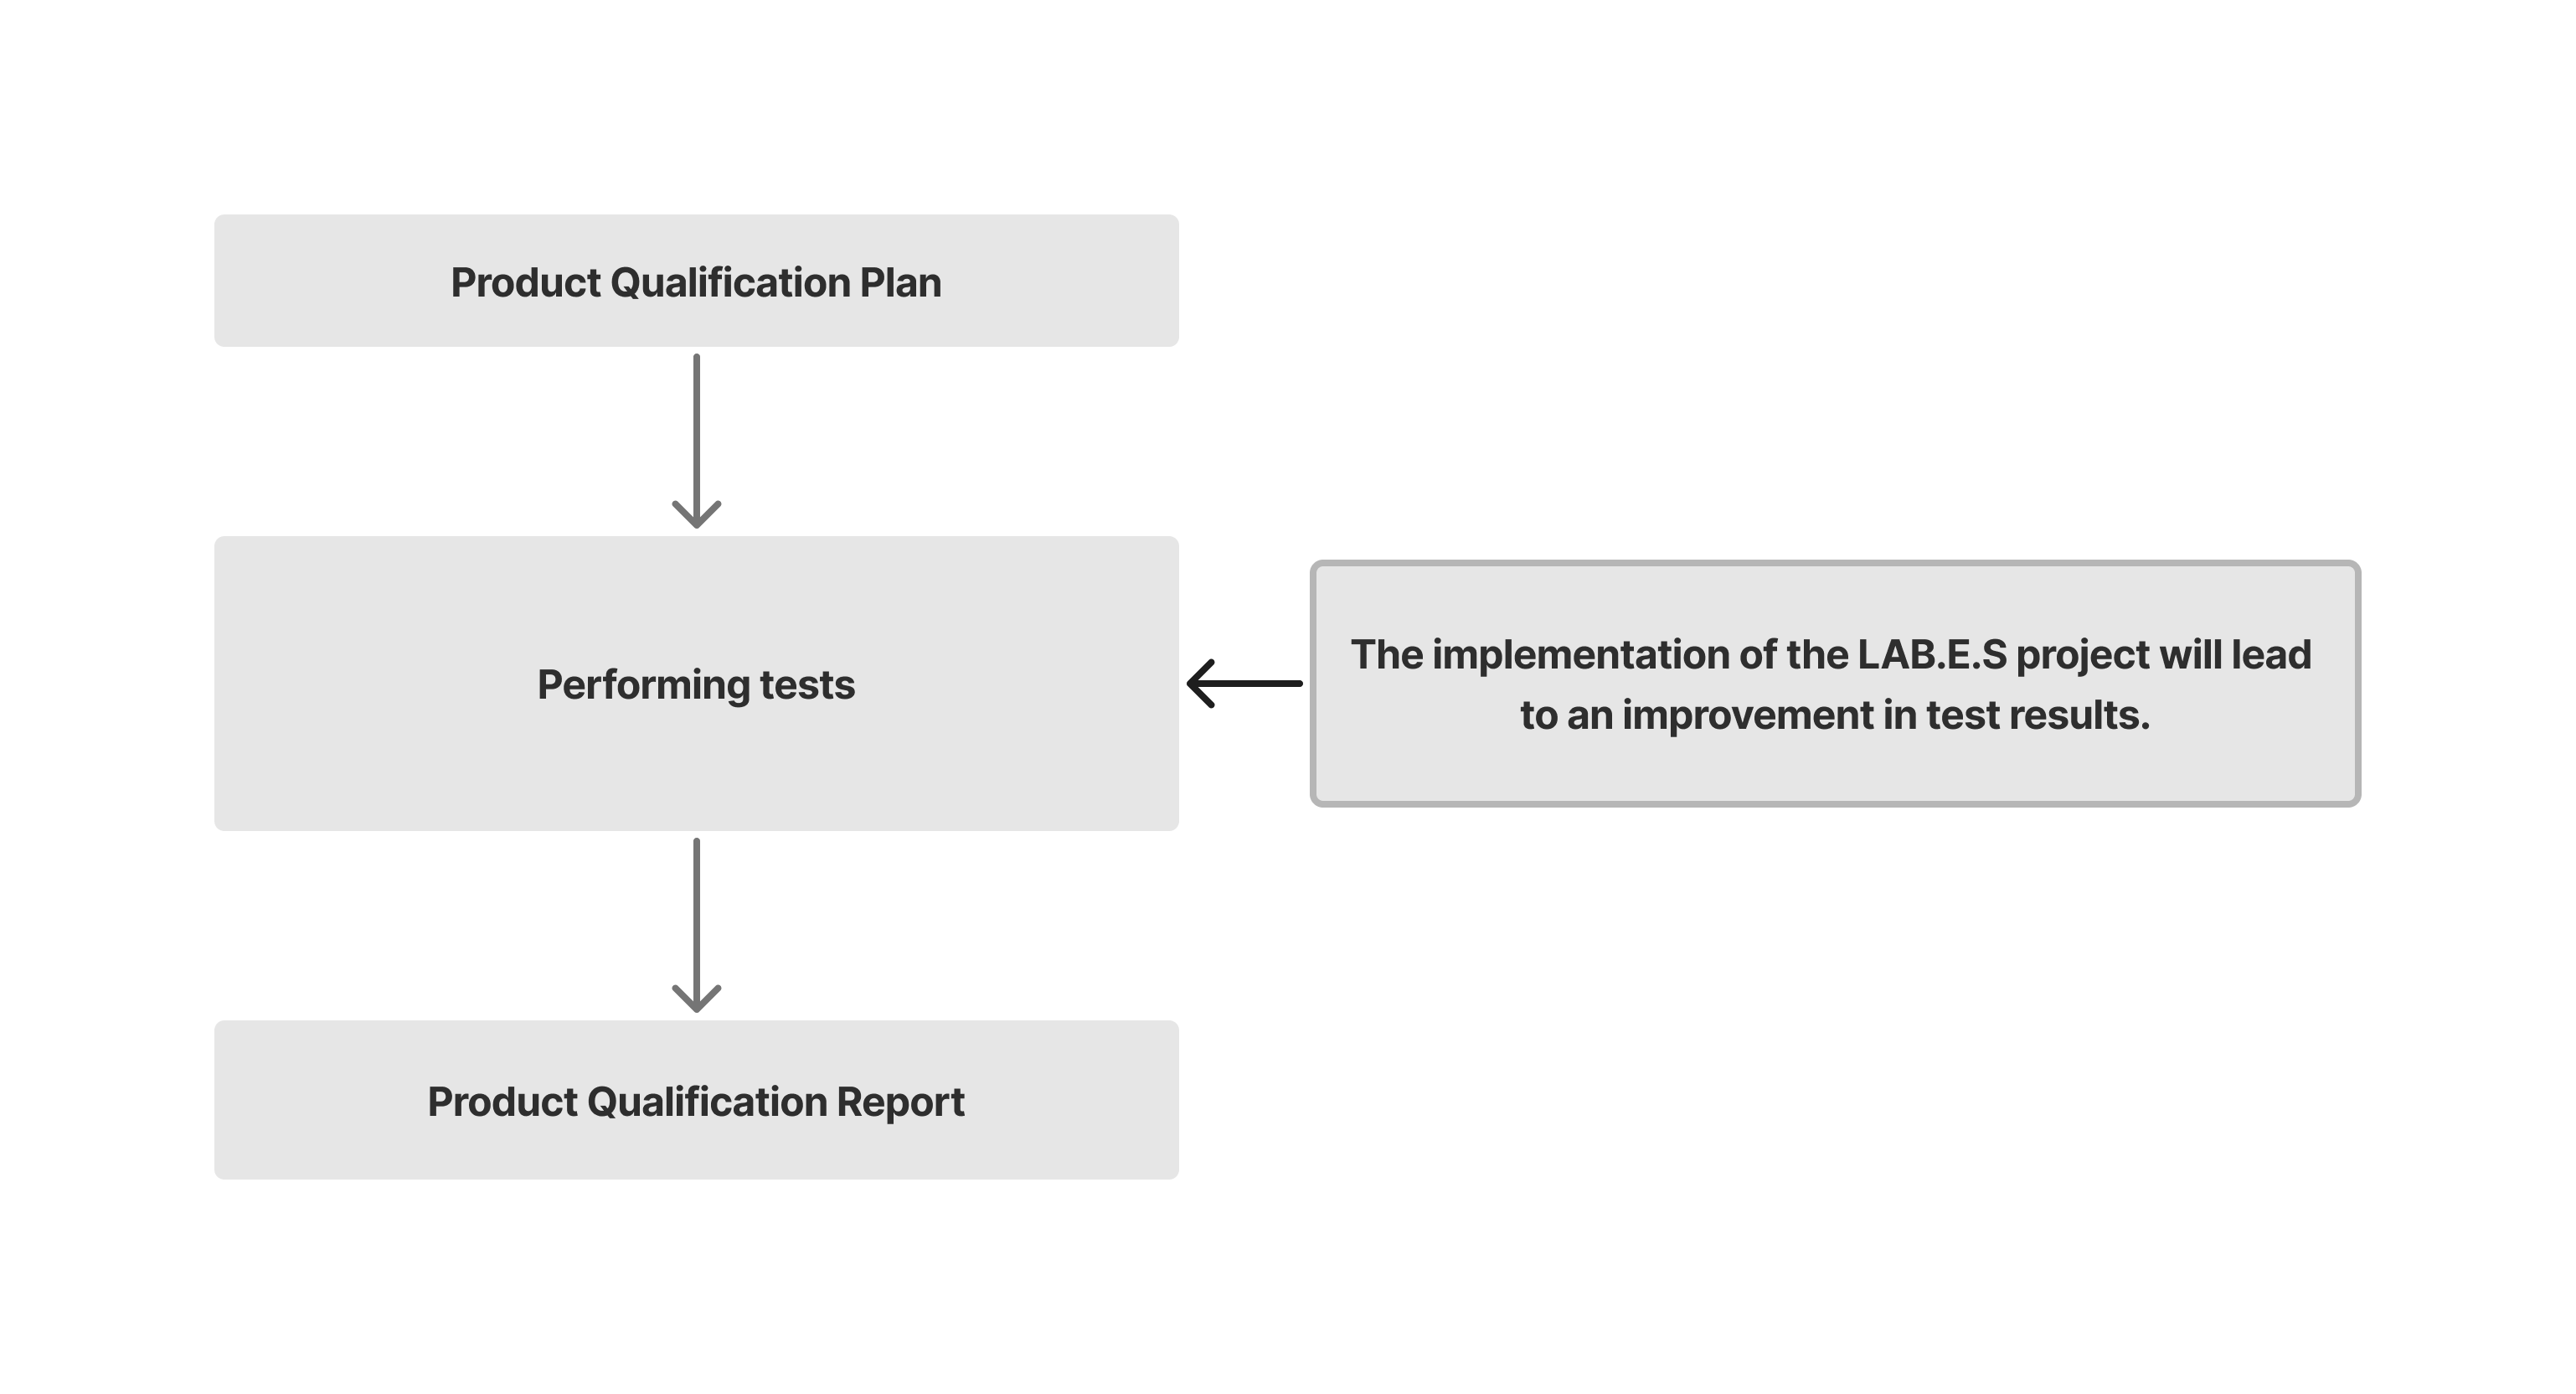
\includegraphics[width=1\textwidth]{chapters/2/img/User Flows (2).png}
    \caption{Somfy Zriba Lab}
    \label{fig:campus}
\end{figure}

\subsection{Exemple d'Application Industrielle existante dans le Site Somfy}

MES is a production planning and supervision tool and these are the key characteristics of SOMFY MES:

\begin{enumerate}
\item Create or edit product data: Oversee the development or revision of production-related documentation, data collecting, and parameter configuration.
\item Schedule: To guarantee effective, real-time production, create and update schedules and manage and optimize the production schedule.

\item Produce: Manage the complete manufacturing process, including start-up, production quantity control, and issue resolution, to guarantee company continuity.
\end{enumerate}
\begin{figure}[H]
    \centering
    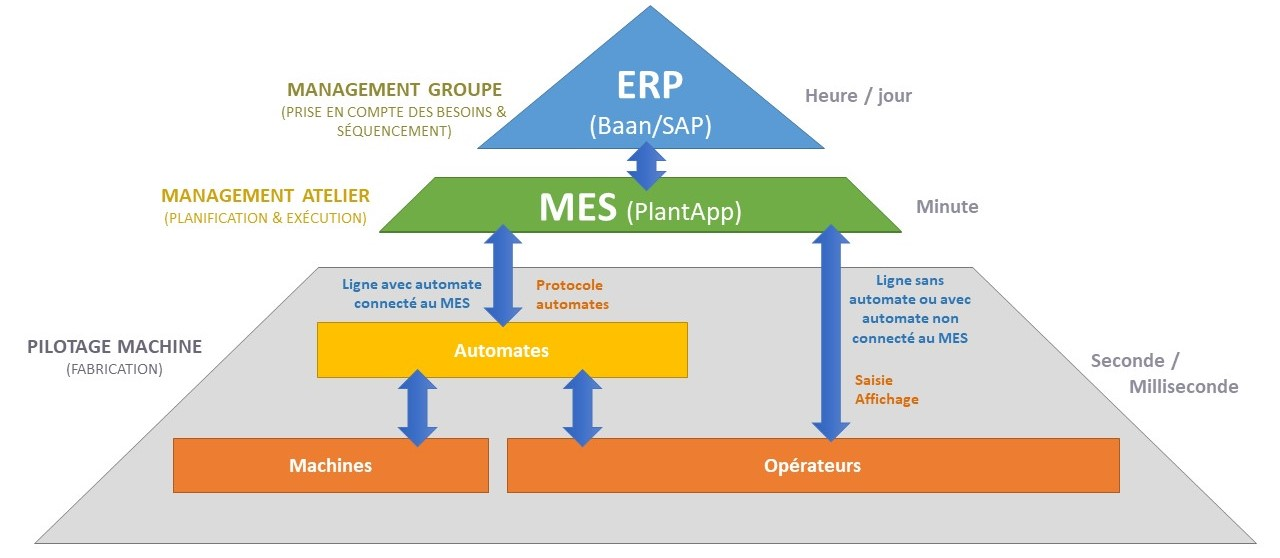
\includegraphics[width=1\textwidth]{chapters/2/img/LES - Molka Abid.jpg}
    \caption{Somfy Zriba Lab}
    \label{fig:campus}
\end{figure}


\subsection{Conclusion de l'Intégration du Digital dans le laboratoire}

The LABES (Laboratory Execution System) application is directly inspired by the MES (Manufacturing Execution System). Just as MES oversees and improves industrial production processes in real time, LABES seeks to convert the laboratory into a completely digitalized and integrated entity.
This development is critical for improving the efficiency, traceability, and quality of laboratory operations, ensuring Somfy's continuing success and increased capacity for innovation.

\section{Etude des besoins}

The LAB.E.S project seeks to provide an innovative platform for real-time monitoring of laboratory operations. This solution will concentrate automated data and offer it to the management team in a clear, structured format. It also aims to automate all administrative papers and handle all laboratory operations.

\subsection{Identification des besoins fonctionnels}
\begin{enumerate}
    \item

Connection to PLCs: To retrieve equipment data in real time, the platform must be able to connect to the laboratory's PLCs.
\item
Continuous supervision: This must allow for continuous tracking of laboratory activities and test results.
\item
Test Subject Sheet Management: Employees must be able to generate and manage test subject sheets directly from the platform.
\item
Data display: Collected data should be freely available and visible on laboratory screens.
\item
A dashboard should pull together all of the collected data, providing management with a clear, unifying picture.
\item
Intuitive User Interface: To make data access and interpretation easier, the platform must have a user-friendly, intuitive, and simple interface.
\item
Data confidentiality and integrity must be ensured by strong security measures.
\end{enumerate}
\subsection{Étude des besoins non fonctionnels}

\begin{enumerate}
\item

Performance: The platform must react swiftly to queries while remaining highly available.

\item
Reliability: It must be resilient, with fail-safe procedures and maximum uptime.

\item
Scalability: The platform must be capable of handling an increase in workload, particularly by including additional test benches and PLCs.

\item
Security:
Security mechanisms must be in place to prevent unwanted access and maintain data integrity.

\item
Compatibility: The platform must be interoperable with various PLC kinds as well as current laboratory systems.

\item
Maintainability: The platform should be simple to manage, with frequent upgrades and enough technical assistance.

\item
Usability: The platform should be simple to use, with an intuitive UI and a quick learning curve.

\item
Portability: It must be flexible to multiple hardware and software infrastructures.
\end{enumerate}

%\subsection{Backlog du produit}
\subsection{Identification des users}
\begin{description}\item[Admin:]\end{description}  The administrator's responsibility is to have broad access and control over the LABES platform. He or she is in charge of overall system administration, which includes configuration, security, and user management.

\begin{description} \item[Pilote de Sujet:]\end{description}  The subject manager is responsible for supervising and coordinating specialized laboratory operations related to a given test subjects and projects.


\subsection{Use case {\&} Validation Case}
Use Cases define the specific interactions between users and the system. They specify the actions that users may take on the site.
Validation Cases are required to guarantee that each Use Case performs as expected. They contain verification processes to ensure that functionality fulfills the specifications and is properly implemented.
\begin{figure}[H]
    \centering
    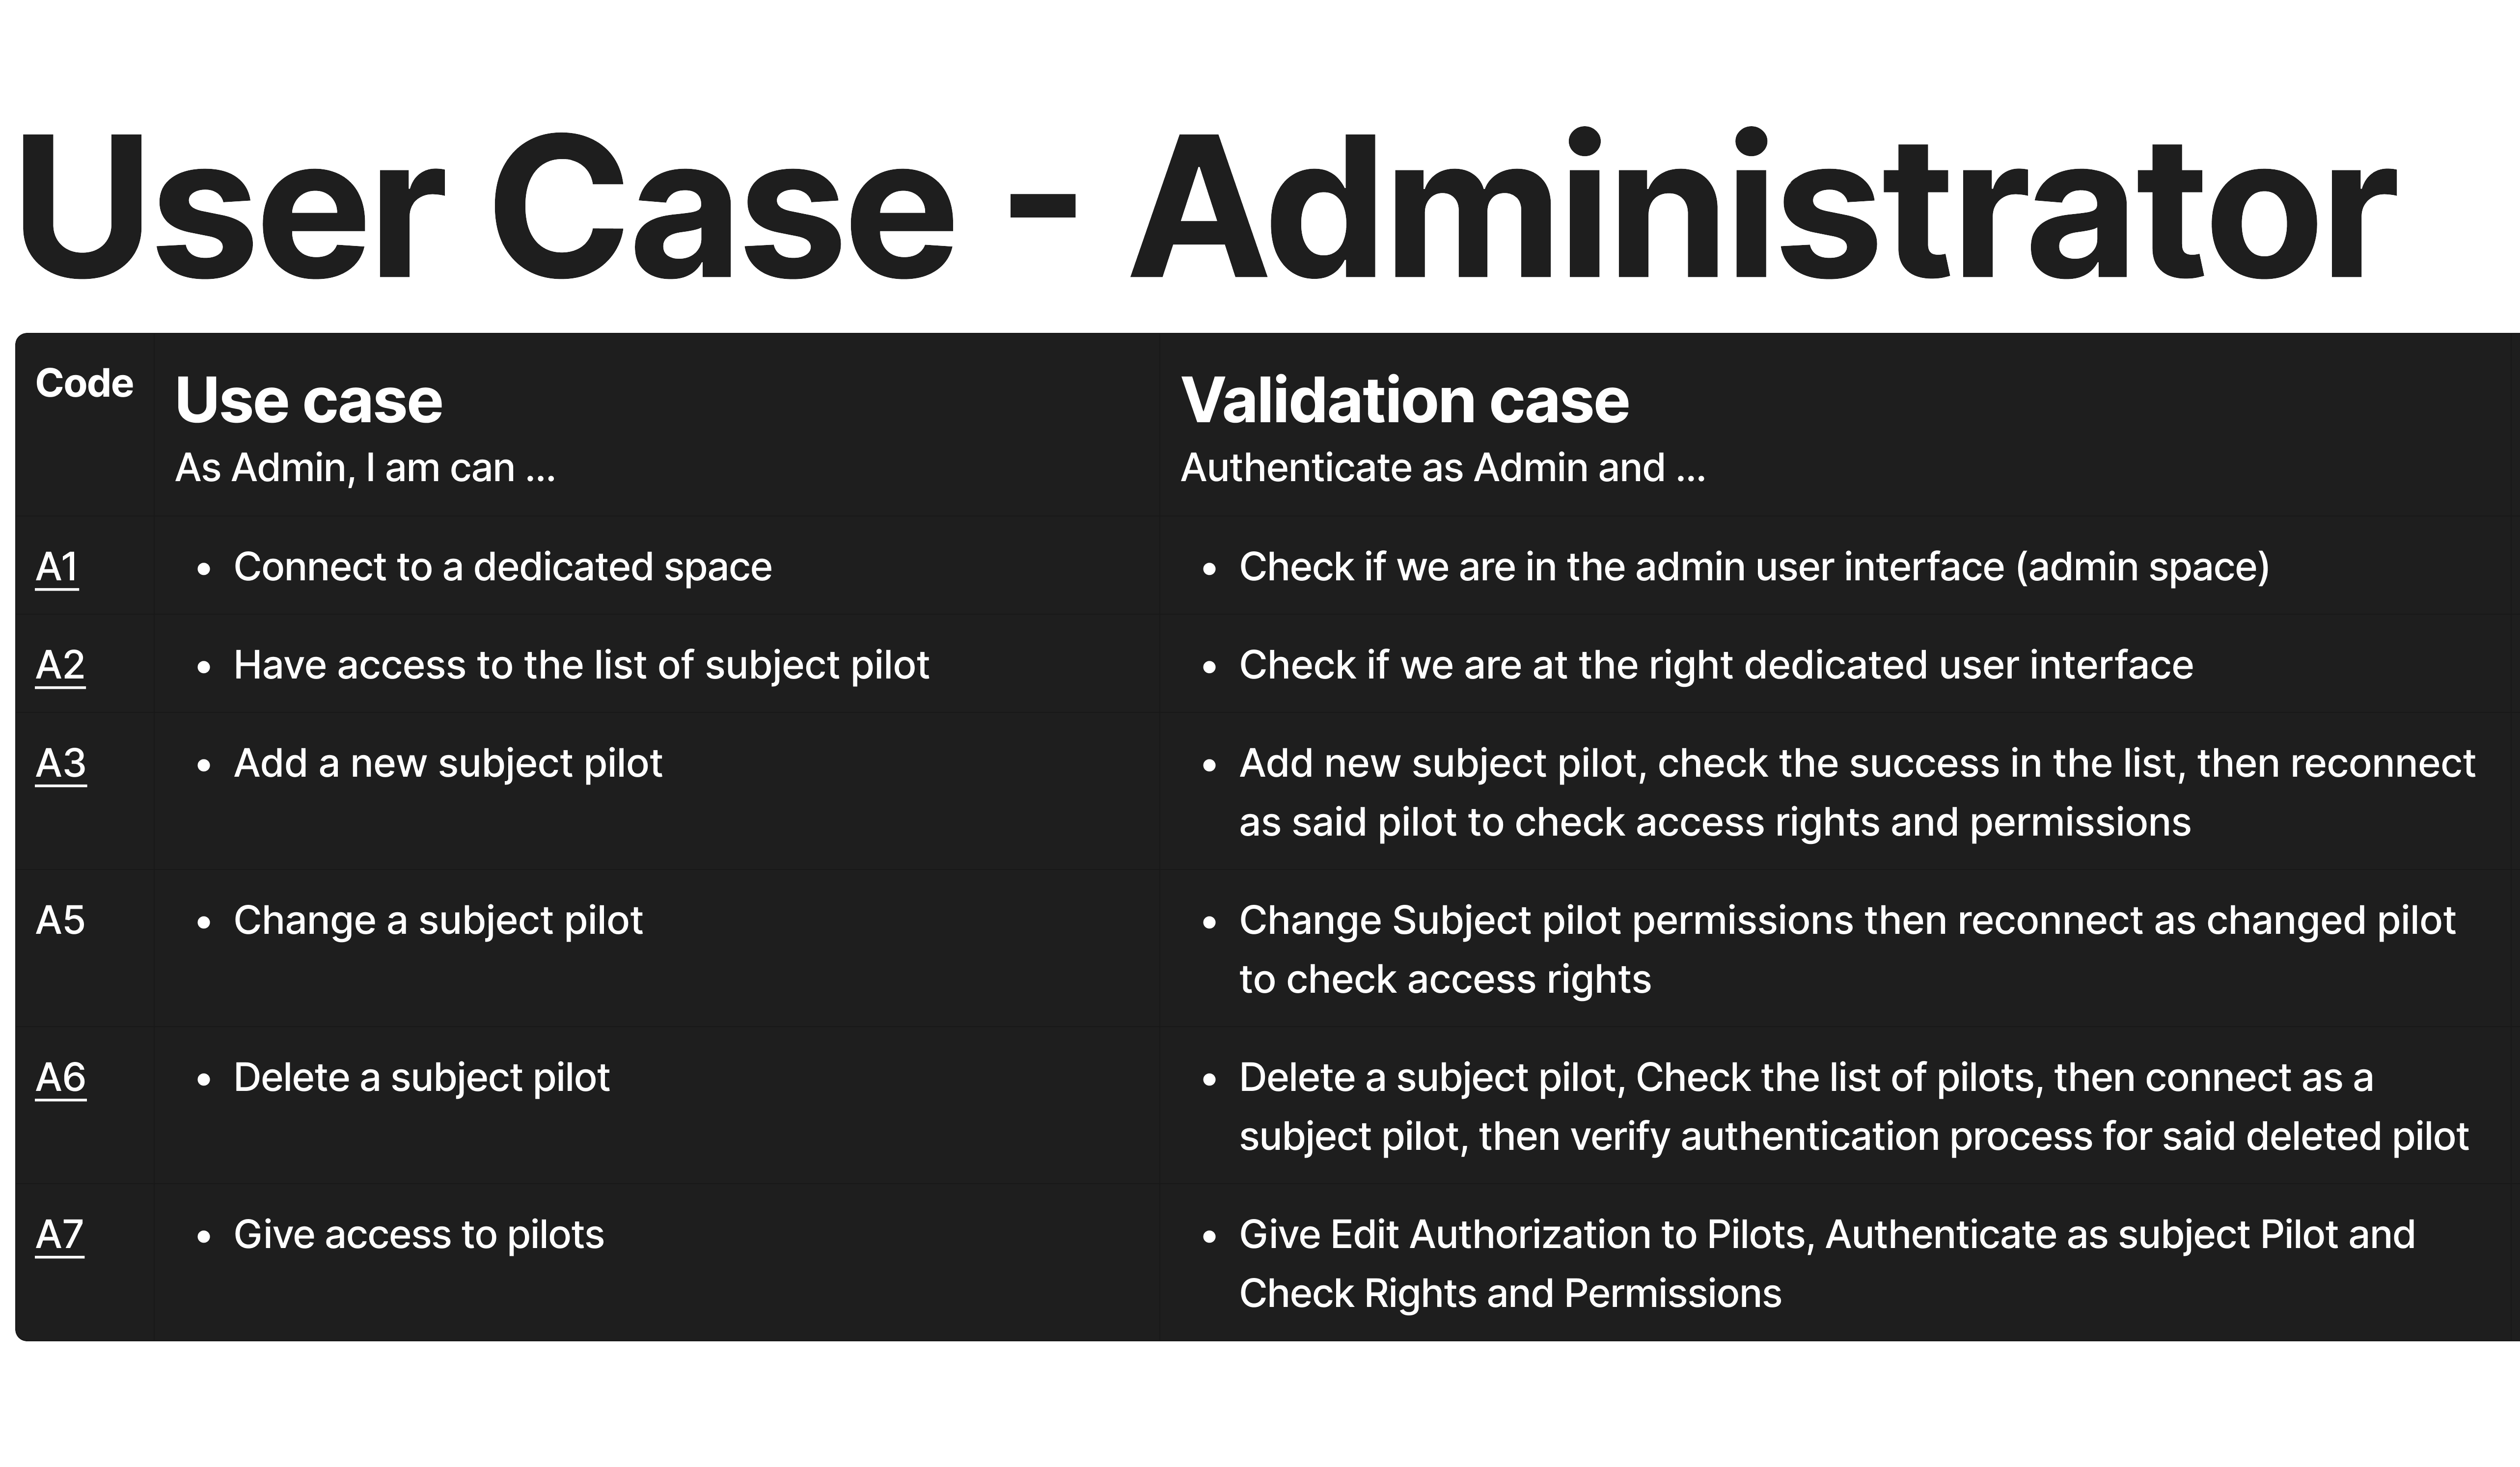
\includegraphics[width=1.1\textwidth]{chapters/2/img/use case.png}
    \caption{Use Case}
    \label{fig:campus}
\end{figure}
\begin{figure}[H]
    \centering
    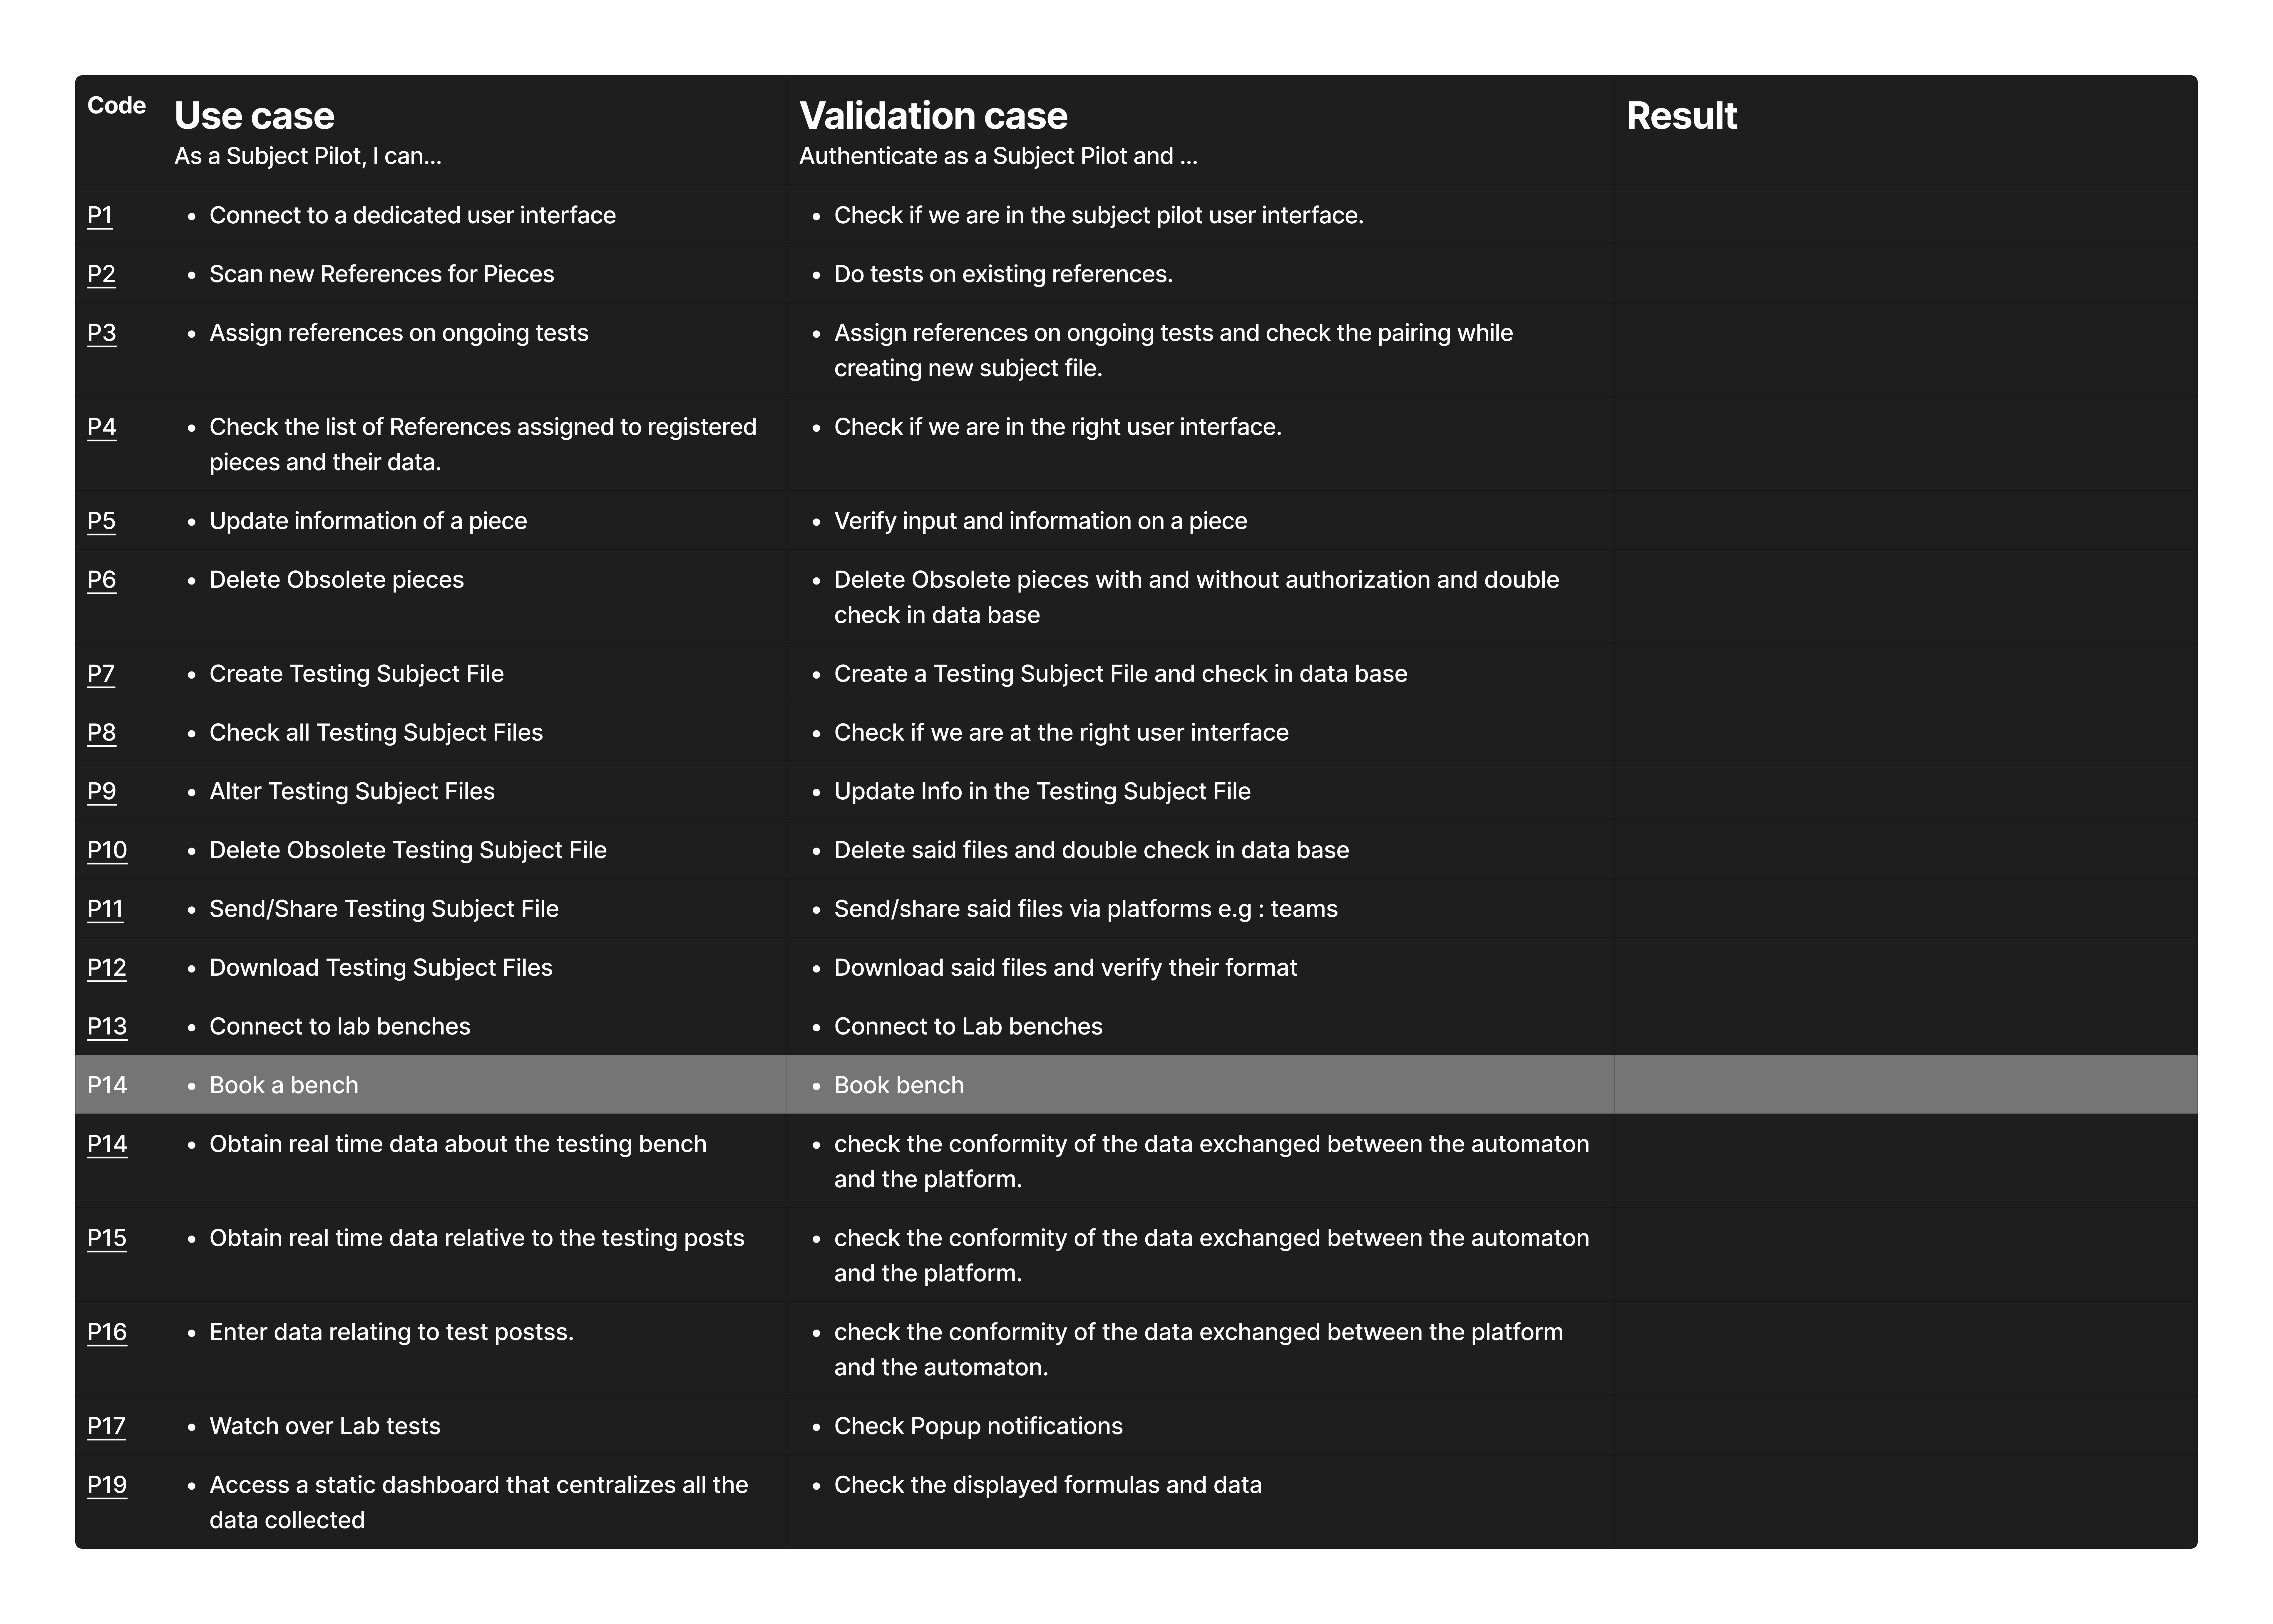
\includegraphics[width=1.\textwidth]{chapters/2/img/1.png}
    \caption{Use Case}
    \label{fig:campus}
\end{figure}

\subsection{User Flow}
A User Flow is a graphic representation of the steps a user takes to achieve a given objective on the platform. It specifies all of the processes, interactions, and decisions that the user must make to complete an action.


\subsubsection {Utilité des User Flow}

\begin{description} \item[Compréhension du parcours utilisateur :]\end{description} 
Understanding the user journey: User flows assist in visualizing and comprehending the path that the user travels through the interface, hence identifying possible friction points.
\begin{description} \item[Amélioration de l'expérience utilisateur :]\end{description} 
Designers can enhance the experience by mapping user flows and making use of each stage.
\begin{description} \item[Communication claire :]\end{description} 
User flows serve as a guide for developers, designers, and other clients, ensuring that everyone understands how users will interact with the system.
\begin{description} \item[Identification des besoins fonctionnels :]\end{description} 
They help specify the functionality needed at each stage of the user experience, ensuring that the application satisfies user expectations.

\subsubsection {Composants d'un User Flow}

\begin{description}\item[Administrateur:]\end{description} 
\begin{itemize}
  \item Entry points: These are the pages where users start their journey, such as the home or login page.
  \item Steps: Each interaction or action taken by the user, such as clicking a button or completing a form.
  \item Decisions: The different options or pathways open to the user, such as whether to register or log in.
  \item Exit points: The points at which the user achieves his goal or quits the journey, such as when logging out.
\end{itemize}
\begin{figure}[H]
    \centering
    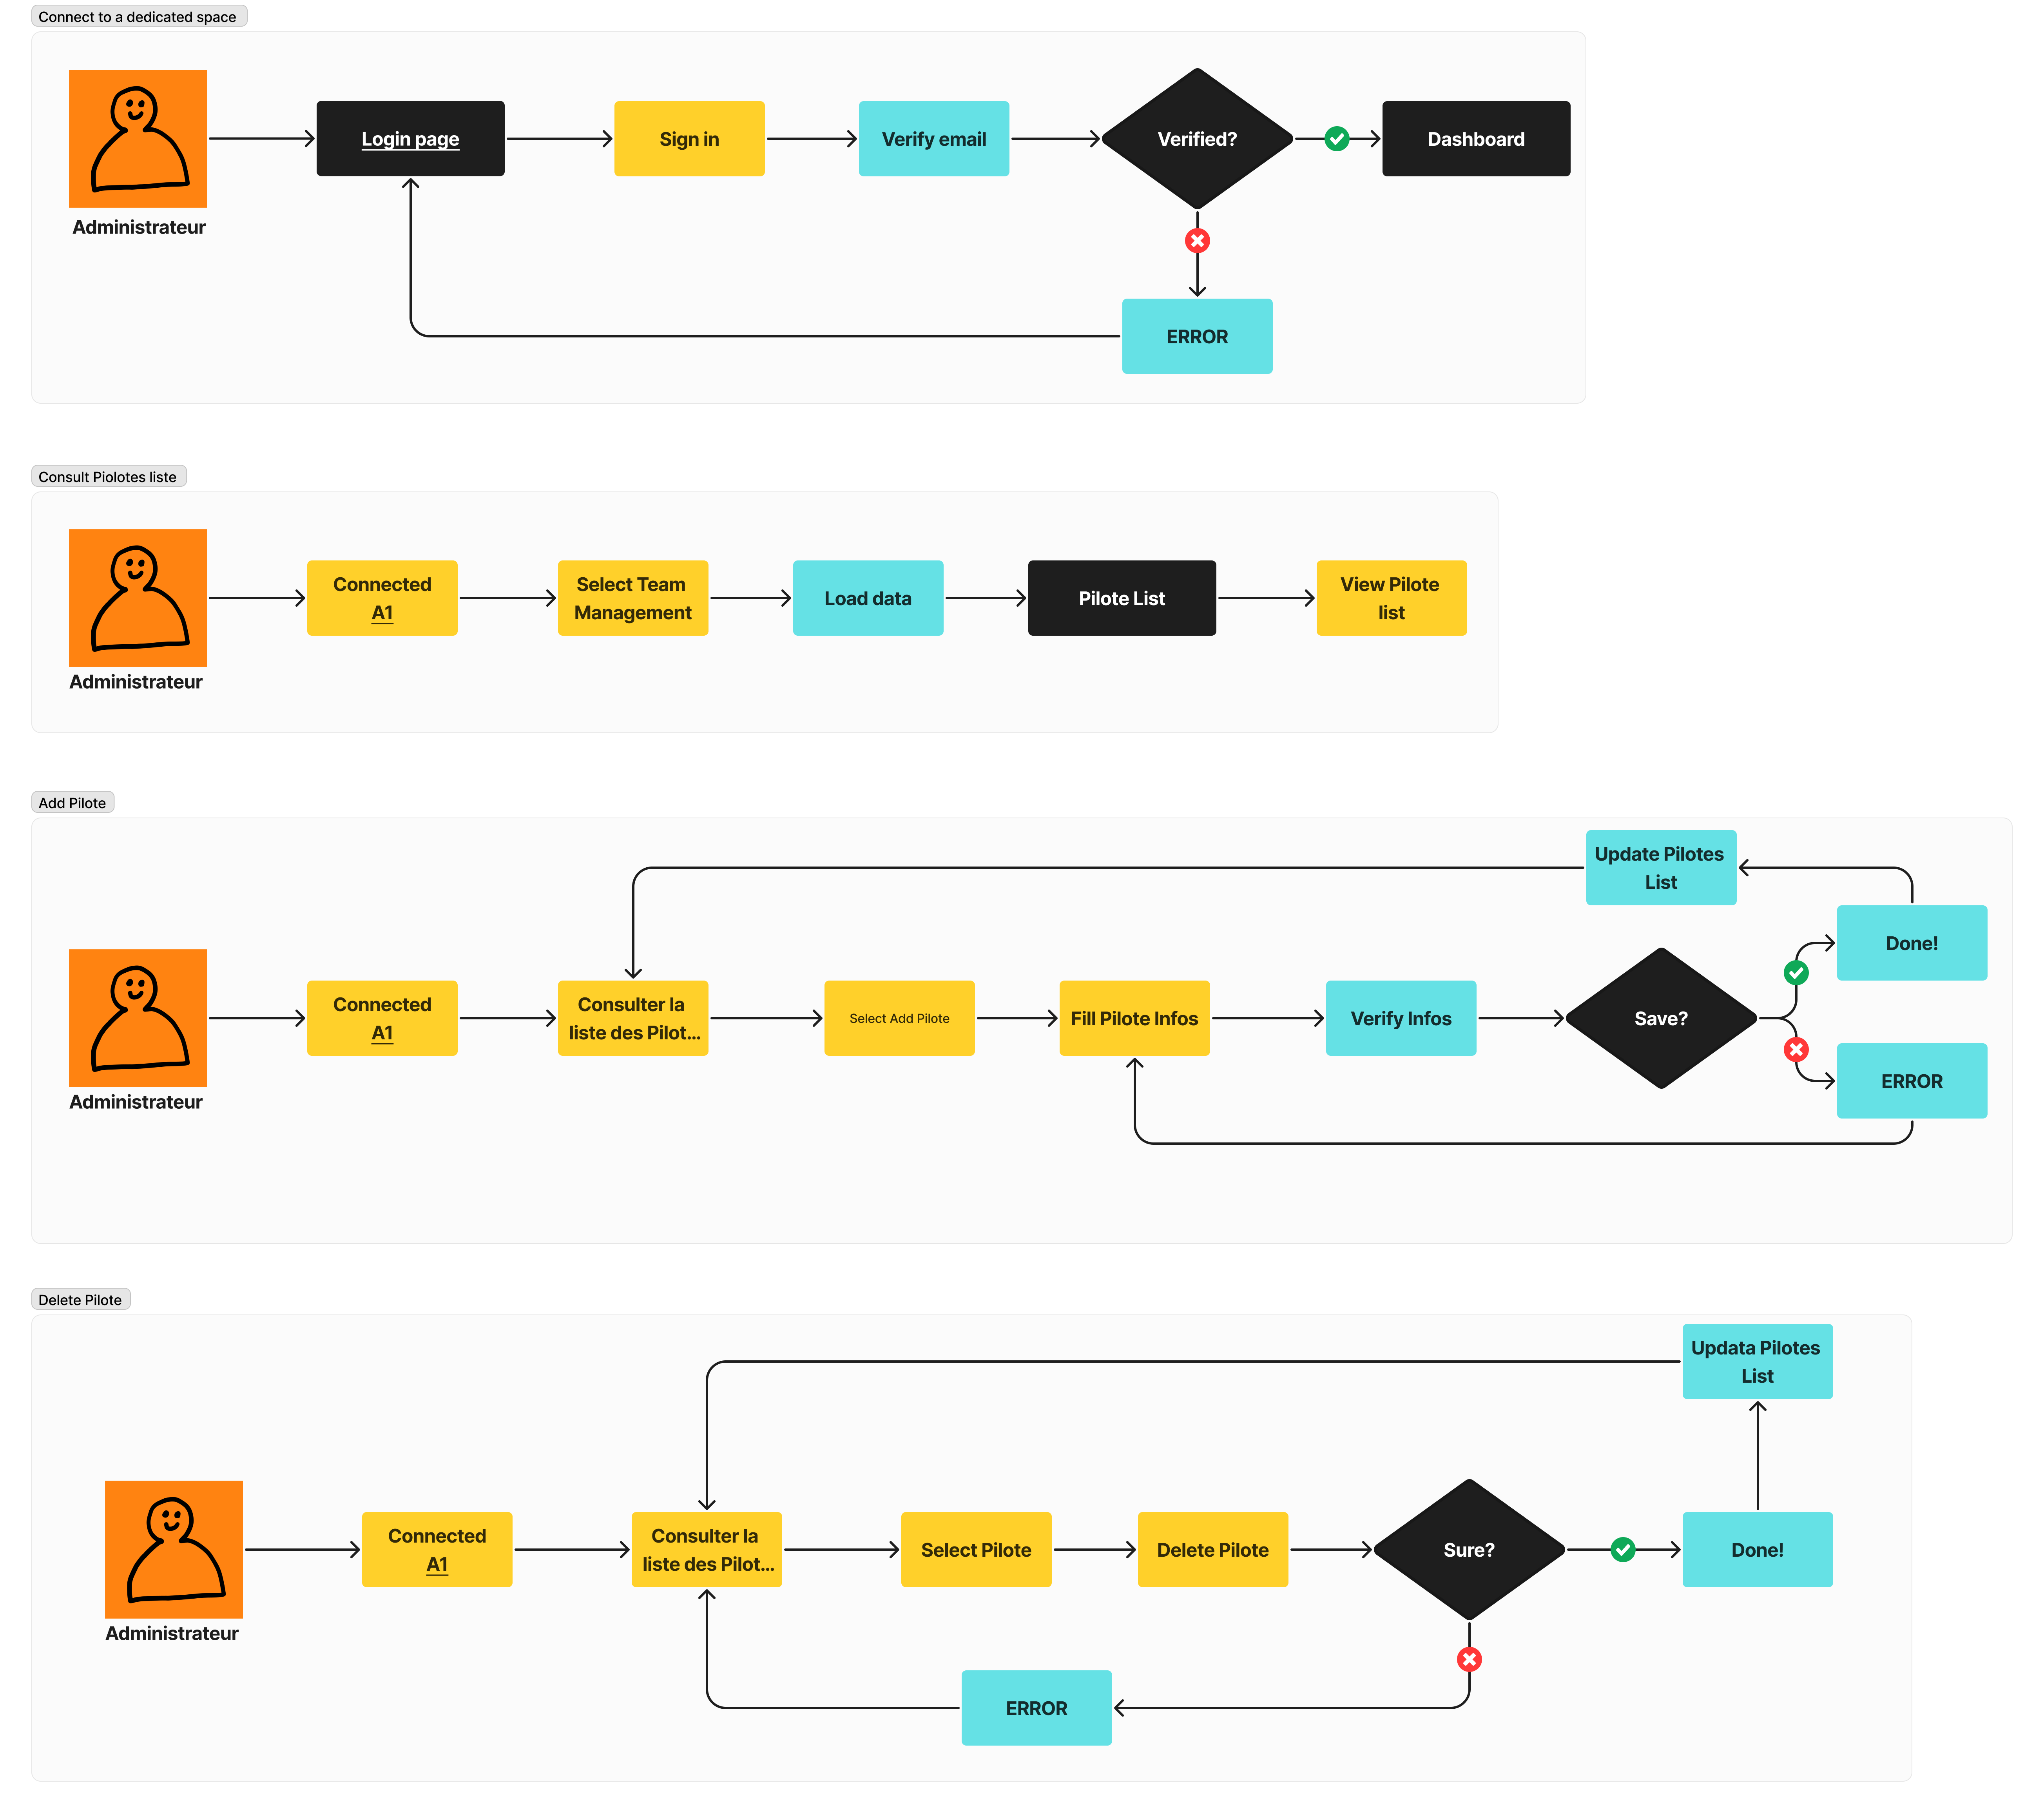
\includegraphics[width=1\textwidth]{chapters/2/img/2.png}
    \caption{Use Case}
    \label{fig:campus}
\end{figure}


\begin{figure}[H]
    \centering
    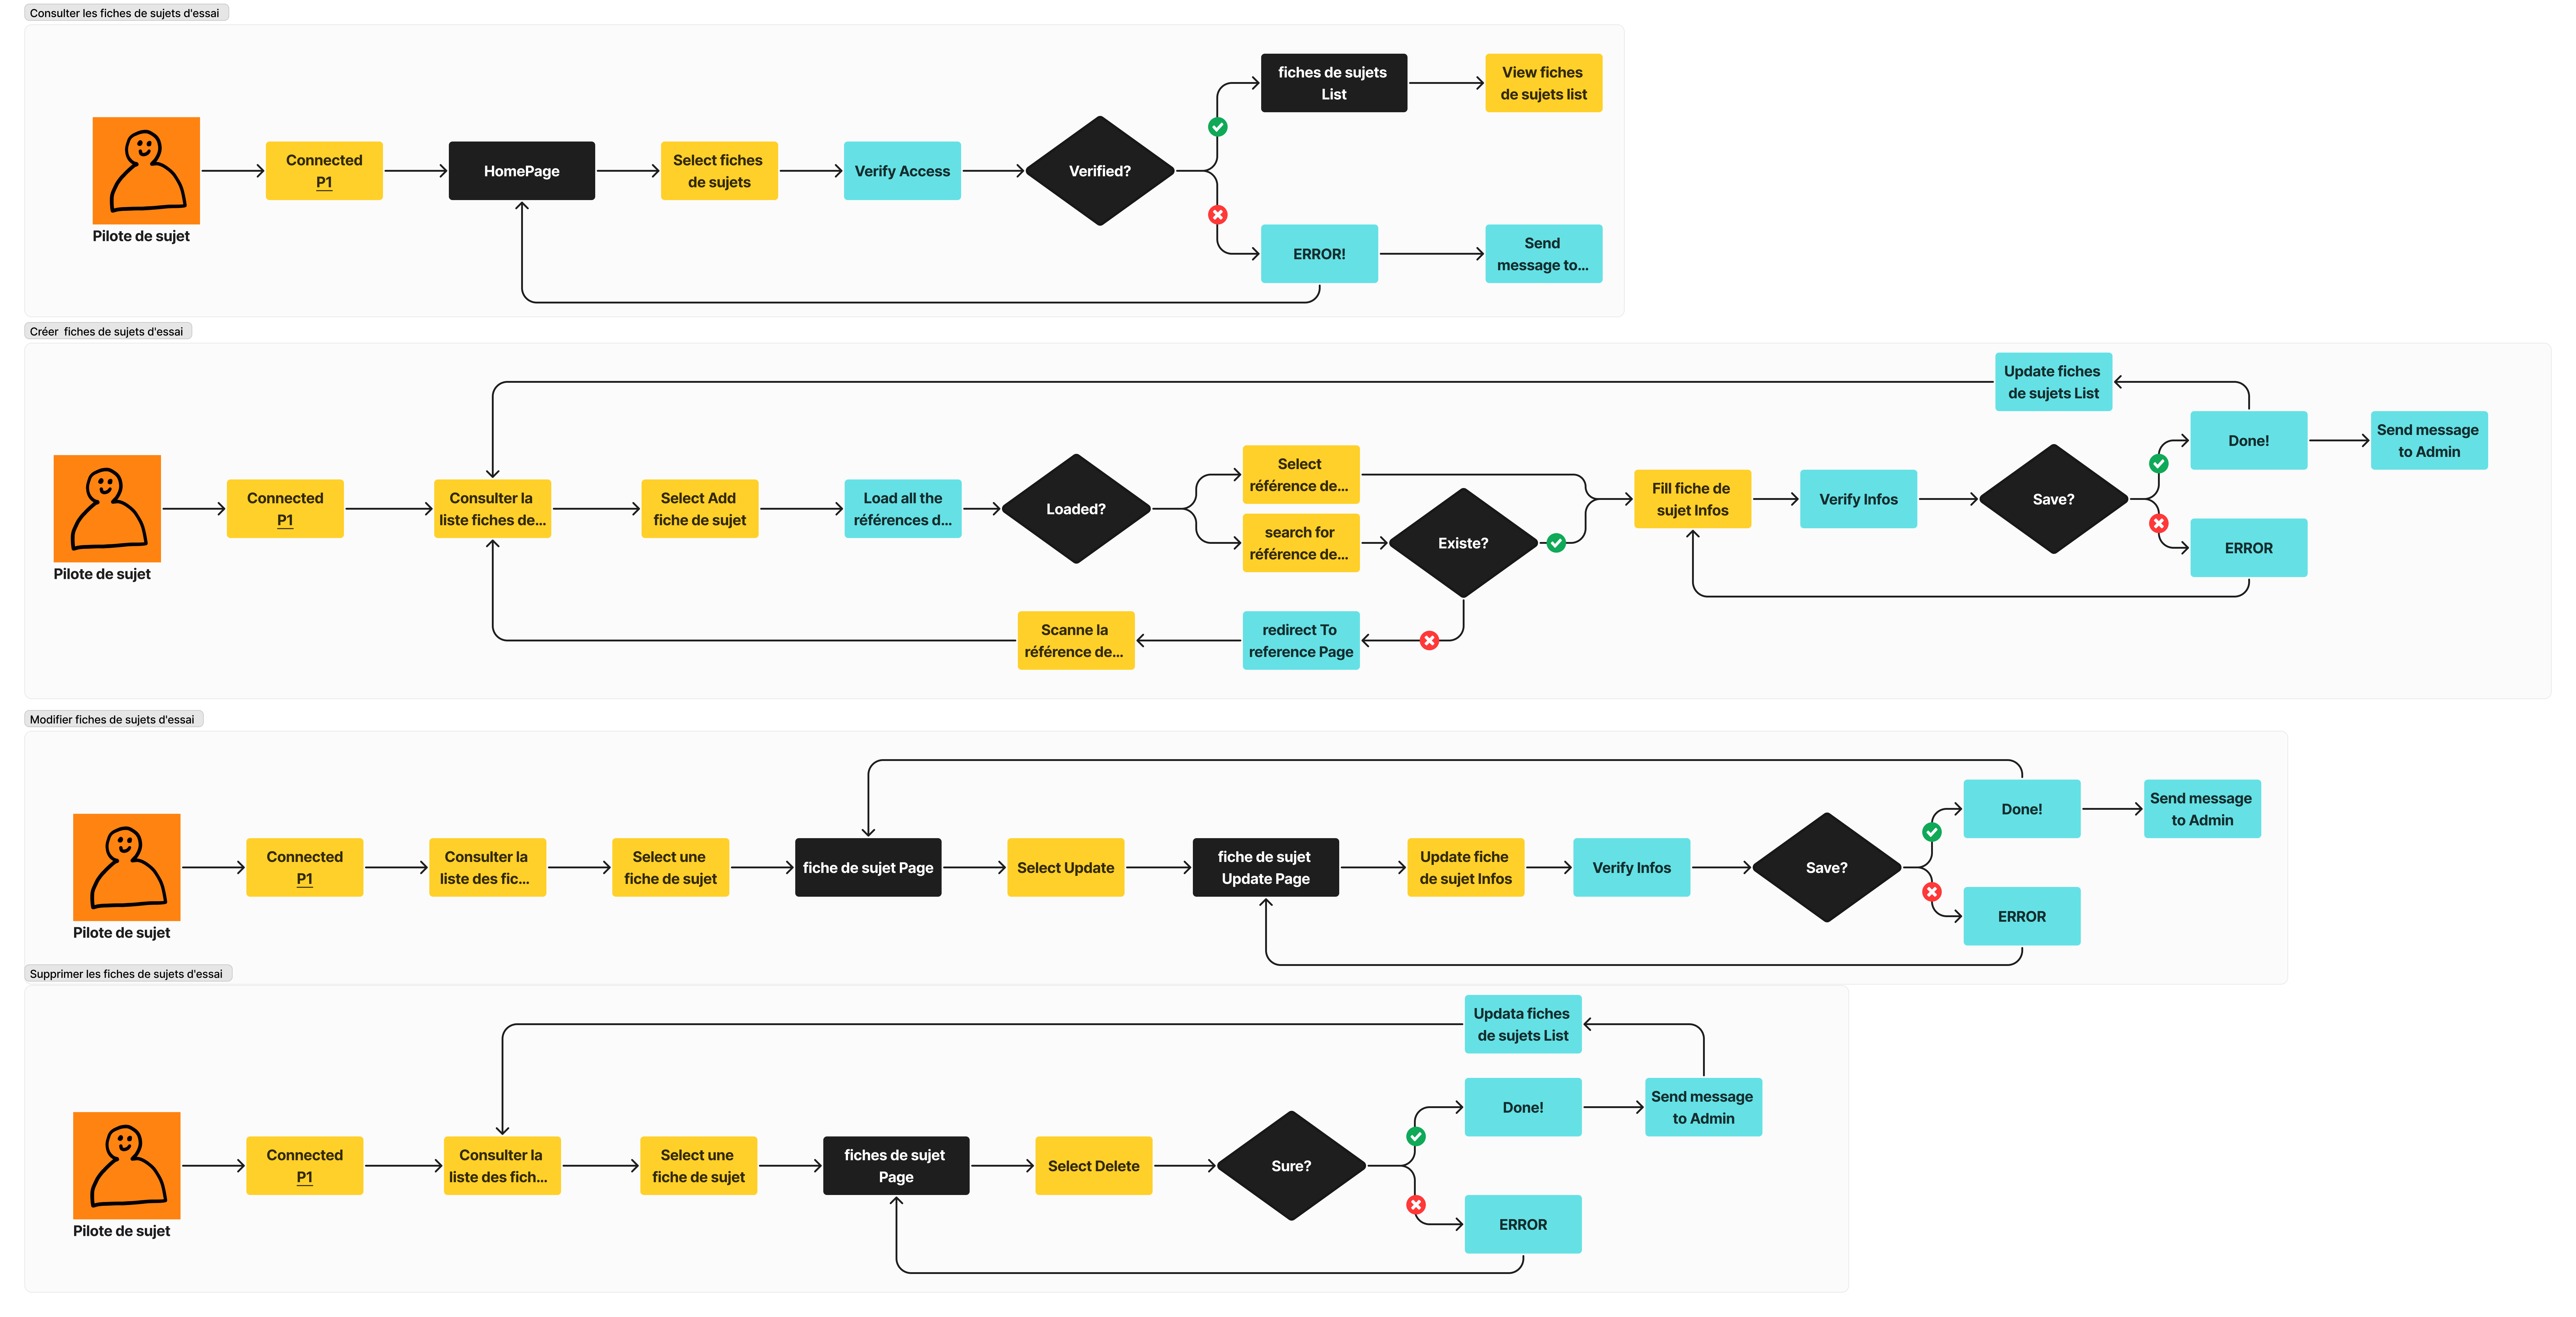
\includegraphics[width=1.5\textwidth, angle=90]{chapters/2/img/3.png}
    \caption{Use Case}
    \label{fig:campus}
\end{figure}
\begin{figure}[H]
    \centering
    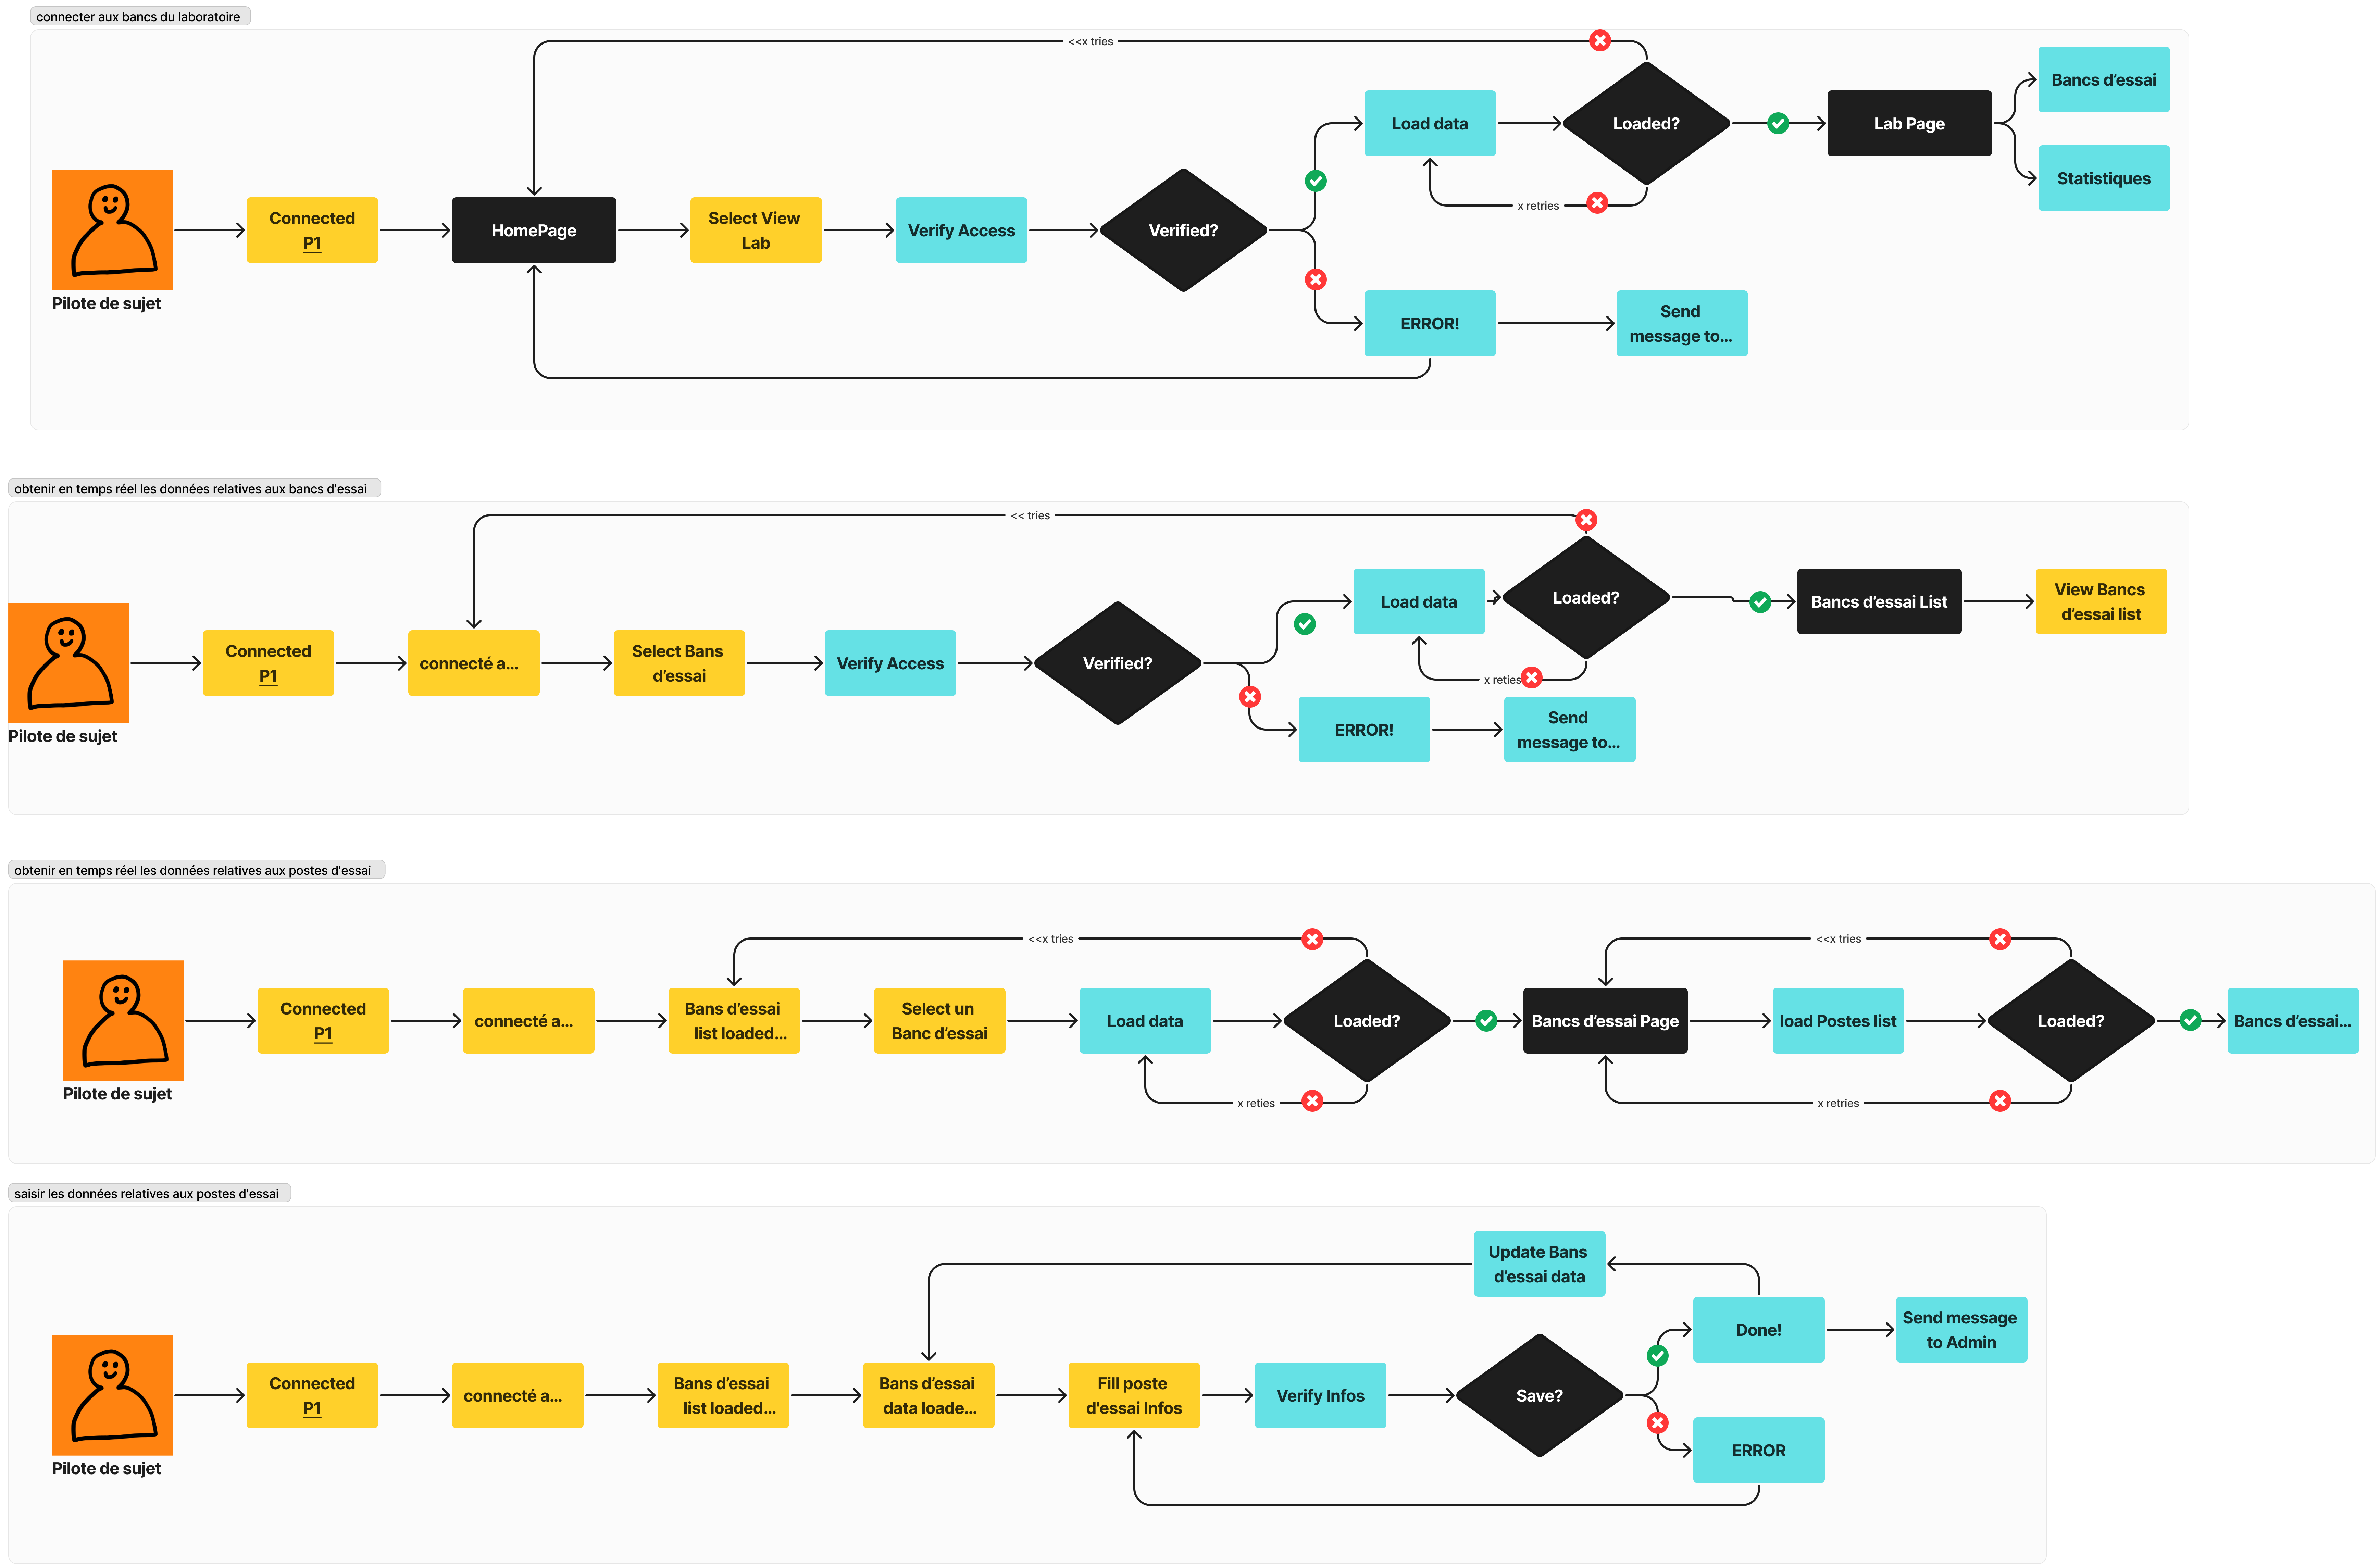
\includegraphics[width=1.5\textwidth, angle=90]{chapters/2/img/4.png}
    \caption{Use Case}
    \label{fig:campus}
\end{figure}
%(par exemple, confirmation d'achat, déconnexion).
\end
\section{Conclution}
The case study, needs analysis, user identification, use cases, and user flows are all critical stages in the design and development of the LABES platform. The case study and needs analysis clearly identified the project's particular requirements. The identification of users, namely the roles of administrator and the subject manager,guaranteed that features were perfectly linked with each unit's expectations and duties. Use cases described the exact functions that users required to be able to do, whereas user flows depicted the user path to maximize the experience and reduce friction points. When these parts are combined cohesively, they result in a well-designed, intuitive platform capable of successfully reacting to users' operational and strategic requirements.

% Part 3
\part{Hardware}
\chapter{Introduction}
As part of the LAB.E.S initiative, it became evident that the laboratory was experiencing a lack of communication. To address this issue, particular consideration was given to hardware design, which included the existing PLCs and their interactions. This section discusses the steps made to improve communication, the features of the available tools, and the changes needed to properly incorporate new functionalities and services.
\clearpage

 Domaines d’application de l’IIoT







\section{Automates Existants et Ajout du Bloc de Communication}
The laboratory's existing Siemens S7-300 PLCs are well-known for their dependability and technical excellence. These controllers, which have been in place since the late 1990s and early 2000s, continue to utilize the same codes today. Although they are well-suited to a range of control and automation activities, their restricted connection posed a significant issue, with the MPI port being the only accessible choice.




\subsection{Caractéristiques principales du S7-300 :}
\begin{itemize}
    \item Input/output modules are adaptable and extensible to meet unique laboratory requirements.
    \item Processor (CPU): A high-performance device capable of processing complicated tasks in real time.
    \item Communication Interfaces: Initially restricted, but require updating to increase connectivity.
\end{itemize}
\subsection{Ajout du Bloc de Communication CP343-1 Lean:}
In order to overcome the S7-300's connectivity constraints, we implemented the CP343-1 Lean communication module. This block has Ethernet connectivity, making it simple to join PLCs with other systems.
The CP 343-1 Lean offers quick, reliable data interchange across several industrial devices, which is an important part of this automation project.

\subsection{Caractéristiques principales du CP343-1 Lean :}

\begin{itemize} 
\item \textbf{Interface Ethernet :} Allows for rapid and reliable connectivity with local area networks (LANs). Supports common protocols including TCP/IP, ISO-on-TCP, and UDP.

\item \textbf{Compatibilité :} Easily integrates with SIMATIC S7-300 PLCs. Simplifies adoption inside existing systems.
\item \textbf{Performance :}
\begin{itemize} 
\item Supports up to 12 simultaneous connections, which fulfills the demands of industrial multitasking situations.
\item Ensures quick transmission, with reaction times ranging from 2.5 to 5 ms, making it excellent for mission important applications.

\end{itemize} 
\item \textbf{Sécurité et Diagnostic :} Fixed MAC address for unique identification on the network.
Includes status LEDs for easy diagnosis of operation and communication.
\item \textbf{Configuration :} Supports flexible configuration via STEP 7 and allows dynamic or manual IP addressing based on network constraints.
\begin{figure}[H]
    \centering
    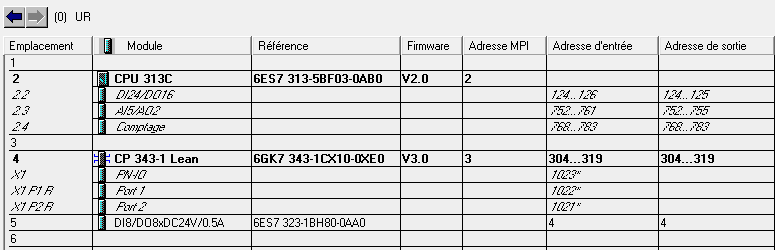
\includegraphics[width=1\textwidth]{chapters/5/img/cp343.png}
    \caption{cp 242-1 LEAN}
    \label{fig:campus}
\end{figure}


\end{itemize}
\section{iBox (Ultra-compact Fanless Embedded Computer)}
\subsection{Définition et Rôle des iBox} 
Les iBox sont des ordinateurs embarqués ultra-compacts et sans ventilateur, spécialement conçus pour des applications industrielles nécessitant fiabilité et robustesse. Ces dispositifs jouent un rôle crucial dans la collecte et le traitement des données des automates.
\subsection{Caractéristiques principales de la série 5000 des Embedded Box PC}

\begin{figure}[H]
    \centering
    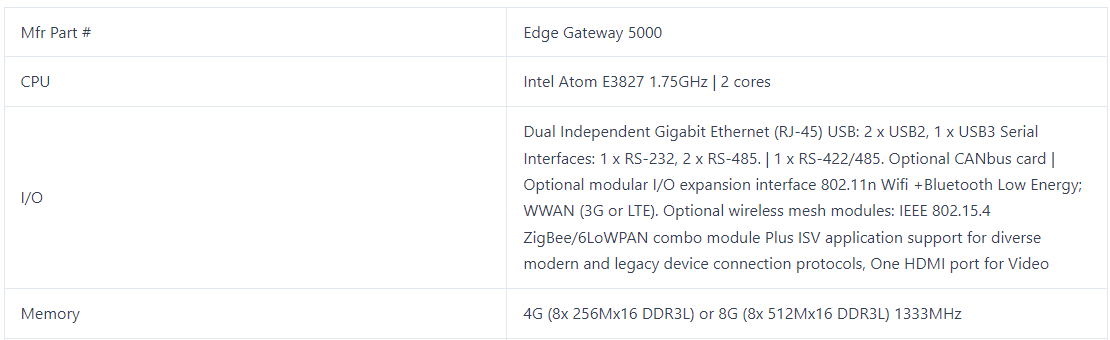
\includegraphics[width=1.1\textwidth]{chapters/5/img/DELLLL.png}
    \caption{Dell Embedded Systems Featuring Intel Atom E3800 Processors}
    \label{fig:campus}
\end{figure}

\subsection{Caractéristiques principales des iBox :}

Compact et Fanless : Conception sans ventilateur, réduisant les risques de défaillance mécanique.
Performance : Capables de traiter des volumes de données importants en temps réel.
Connectivité : Équipés de multiples interfaces pour faciliter la communication avec divers systèmes.
\subsubsection{Applications typiques :}
\begin{itemize}
    \item  Industrial automation involves process control and supervision.
    \item  Fleet monitoring and management, including real-time data collecting and processing. Collecte et traitement des données en temps réel pour une gestion optimisée.
    \item IoT and Edge Computing solutions: Analyze data locally before sending it to a data center or cloud.
\end{itemize}


\section{Test de connectiviter via mqtt }7
\section{Conclution}
The case study, needs analysis, user identification, use cases, and user flows are all critical stages in the design and development of the LABES platform. The case study and needs analysis clearly identified the project's particular requirements. The identification of users, namely the roles of administrator and the subject manager,guaranteed that features were perfectly linked with each unit's expectations and duties. Use cases described the exact functions that users required to be able to do, whereas user flows depicted the user path to maximize the experience and reduce friction points. When these parts are combined cohesively, they result in a well-designed, intuitive platform capable of successfully reacting to users' operational and strategic requirements.

% Part 4
\part{Software}
\chapter{Introduction}
This chapter describes the design and development of the LAB.E.S platform. \\
It emphasizes the strategic decisions and critical actions necessary to convert the laboratory's requirements into a functioning, high-performance platform.
First, the solution's overall layout is detailed, emphasizing its modular and scalable character, which allows harmonic integration of the various components while satisfying the criteria for flexibility and sustainability.
The chapter also describes the database structure, which was built to effectively manage data flows in real time while ensuring the consistency and security of the laboratory's important information.
On a technical level, it describes what steps were taken to construct the frontend and backend. The frontend, built on Figma's UX/UI models, provides an intuitive, high-performance user experience powered by current technologies such as React. Meanwhile, the backend relies on strong, secure services to ensure data processing and interchange across system components.\\
This introduction gives a basic overview which establishes the groundwork for the chapter, which delves into every technical and conceptual element needed in building a solution customized to the laboratory's unique requirements.

\section{Project Architecture Design}

\subsection{System Overview}
The LAB.E.S platform was built using a multi-tier architecture to ensure modularity, scalability, and maintainability. The system is divided into three primary layers:
\begin{itemize}
    \item \textbf{Frontend Layer}: Developed using ReactJS for a responsive and dynamic user interface.
    \item \textbf{Backend Layer}: Built with ASP.NET Core, providing RESTful APIs for communication with the frontend.
    \item \textbf{Data \& Communication Layer}: Handles real-time data exchange using MQTT and stores data in a relational database (SQL Server).
\end{itemize}


\subsection{Microservices Approach}
A microservices architecture was adopted to decouple various system functionalities, allowing independent deployment and scaling of each component. This architecture ensures that the platform remains robust and adaptable as new features are added.
\clearpage


\section{Frontend Development}

\subsection{UI/UX Design Using Figma}
The design of the user interface was initially conceptualized on Figma, focusing on user experience and intuitive navigation. The goal was to create a streamlined interface for laboratory personnel to monitor equipment and data efficiently.

\begin{figure}[H]
    \centering
    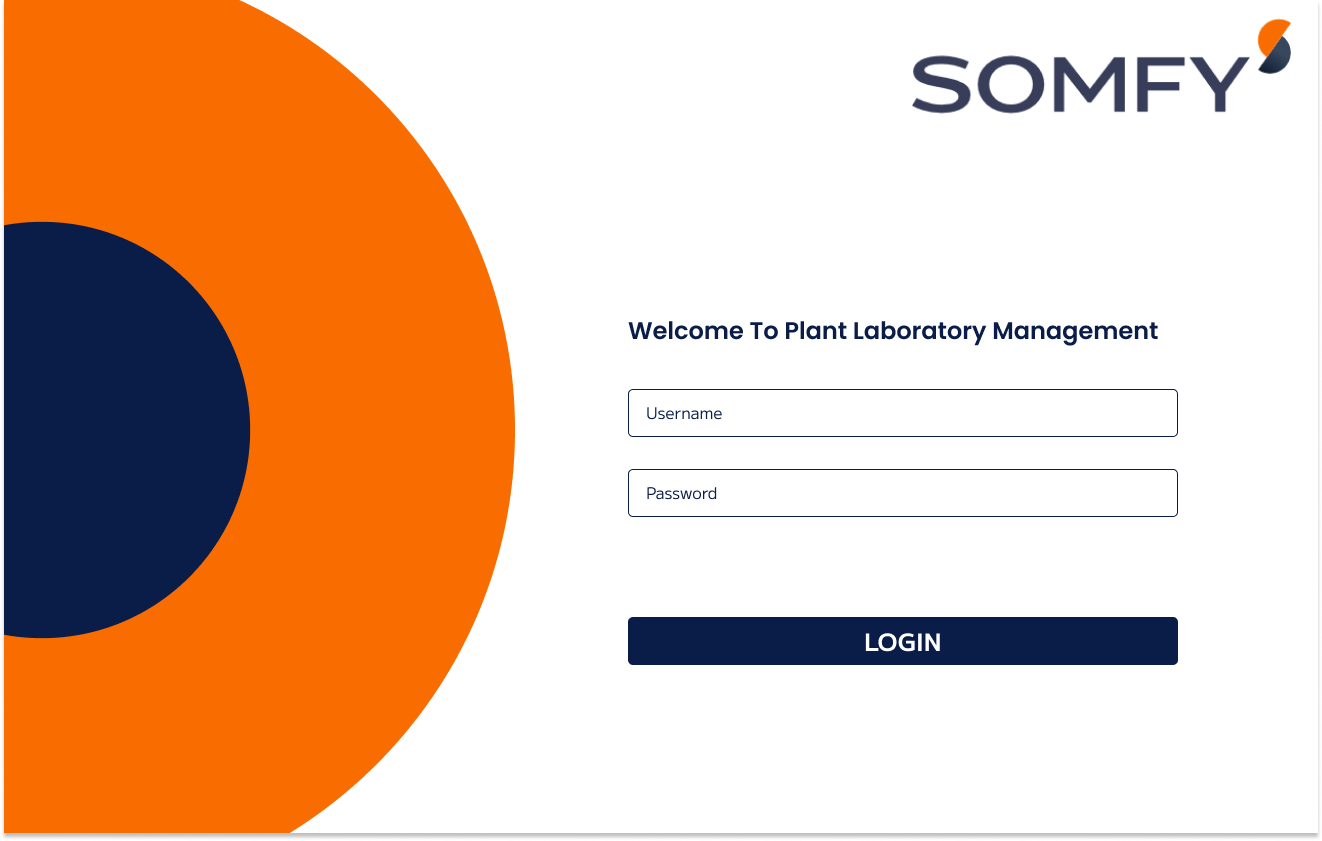
\includegraphics[width=1\textwidth]{chapters/3/img/10.png}
    \caption{cp 242-1 LEAN}
    \label{fig:campus}
\end{figure}

BLABALALALALNA LNNNLLALD

\begin{figure}[H]
    \centering
    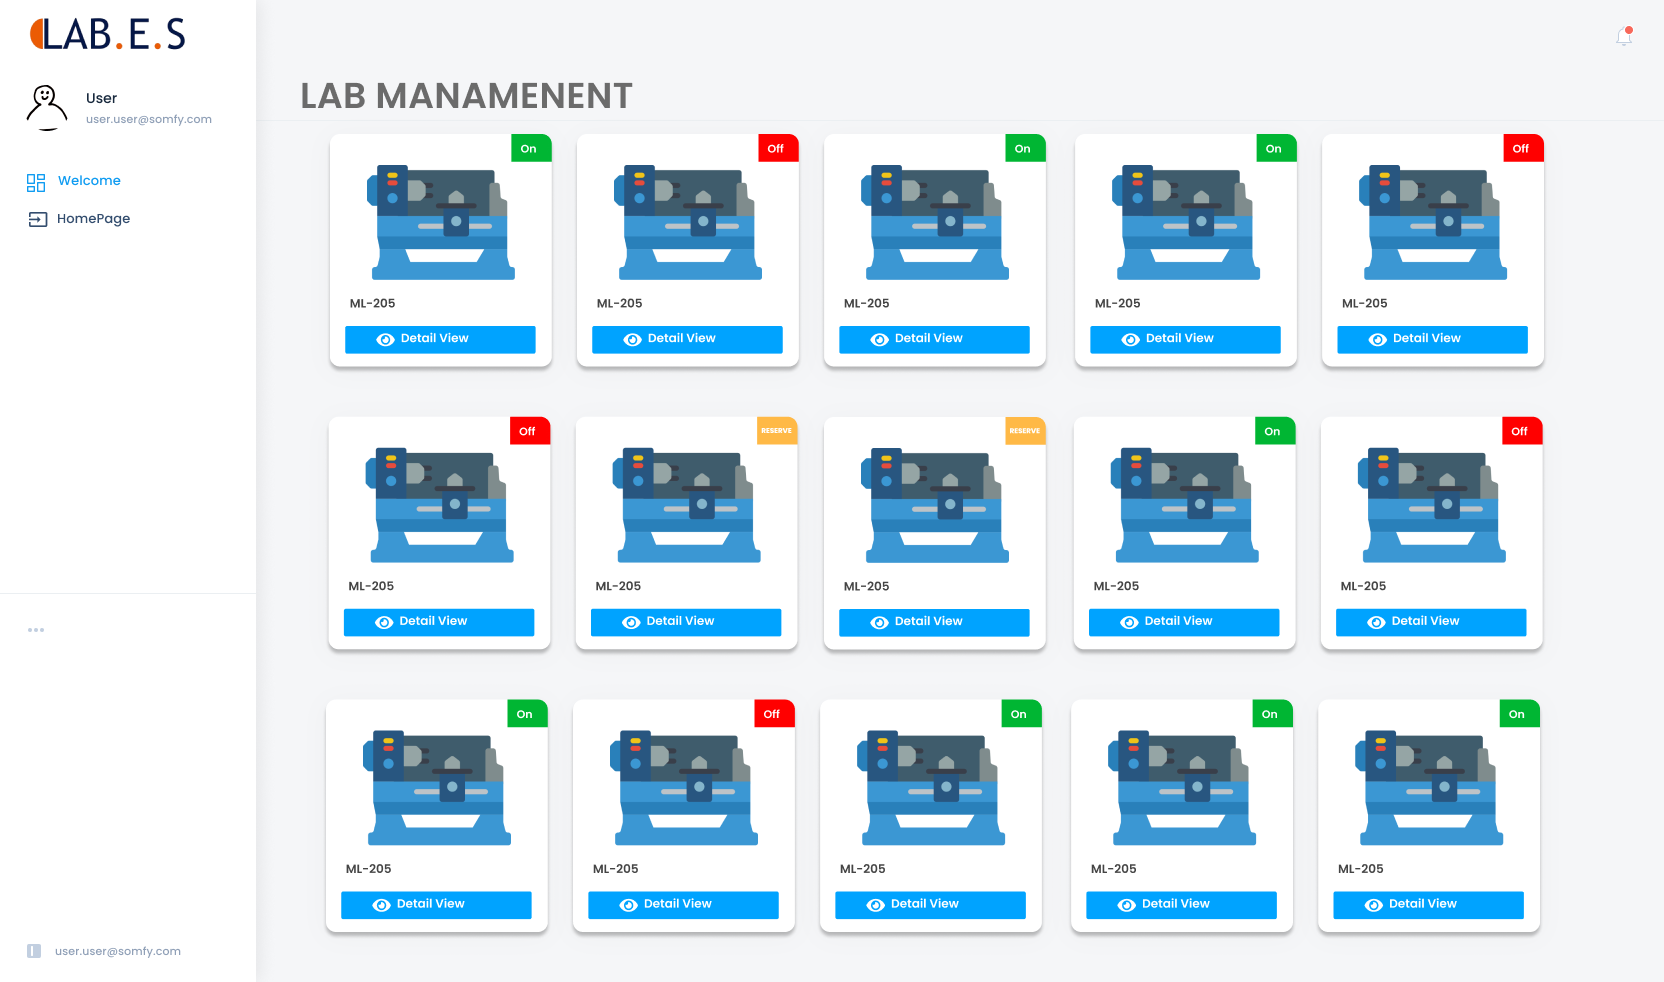
\includegraphics[width=1\textwidth]{chapters/3/img/12.png}
    \caption{cp 242-1 LEAN}
    \label{fig:campus}
\end{figure}



\subsection{ReactJS Implementation}
The frontend was implemented using ReactJS, leveraging its component-based architecture. This allowed for the creation of reusable components, reducing development time. Key features include:
\begin{itemize}
    \item \textbf{Real-Time Data Visualization}: Dynamic dashboards to monitor lab operations.
    \item \textbf{Interactive Forms}: Efficient data entry and equipment management.
    \item \textbf{Responsive Design}: Ensuring compatibility across devices, from desktops to tablets.
\end{itemize}


\begin{figure}[H]
    \centering
    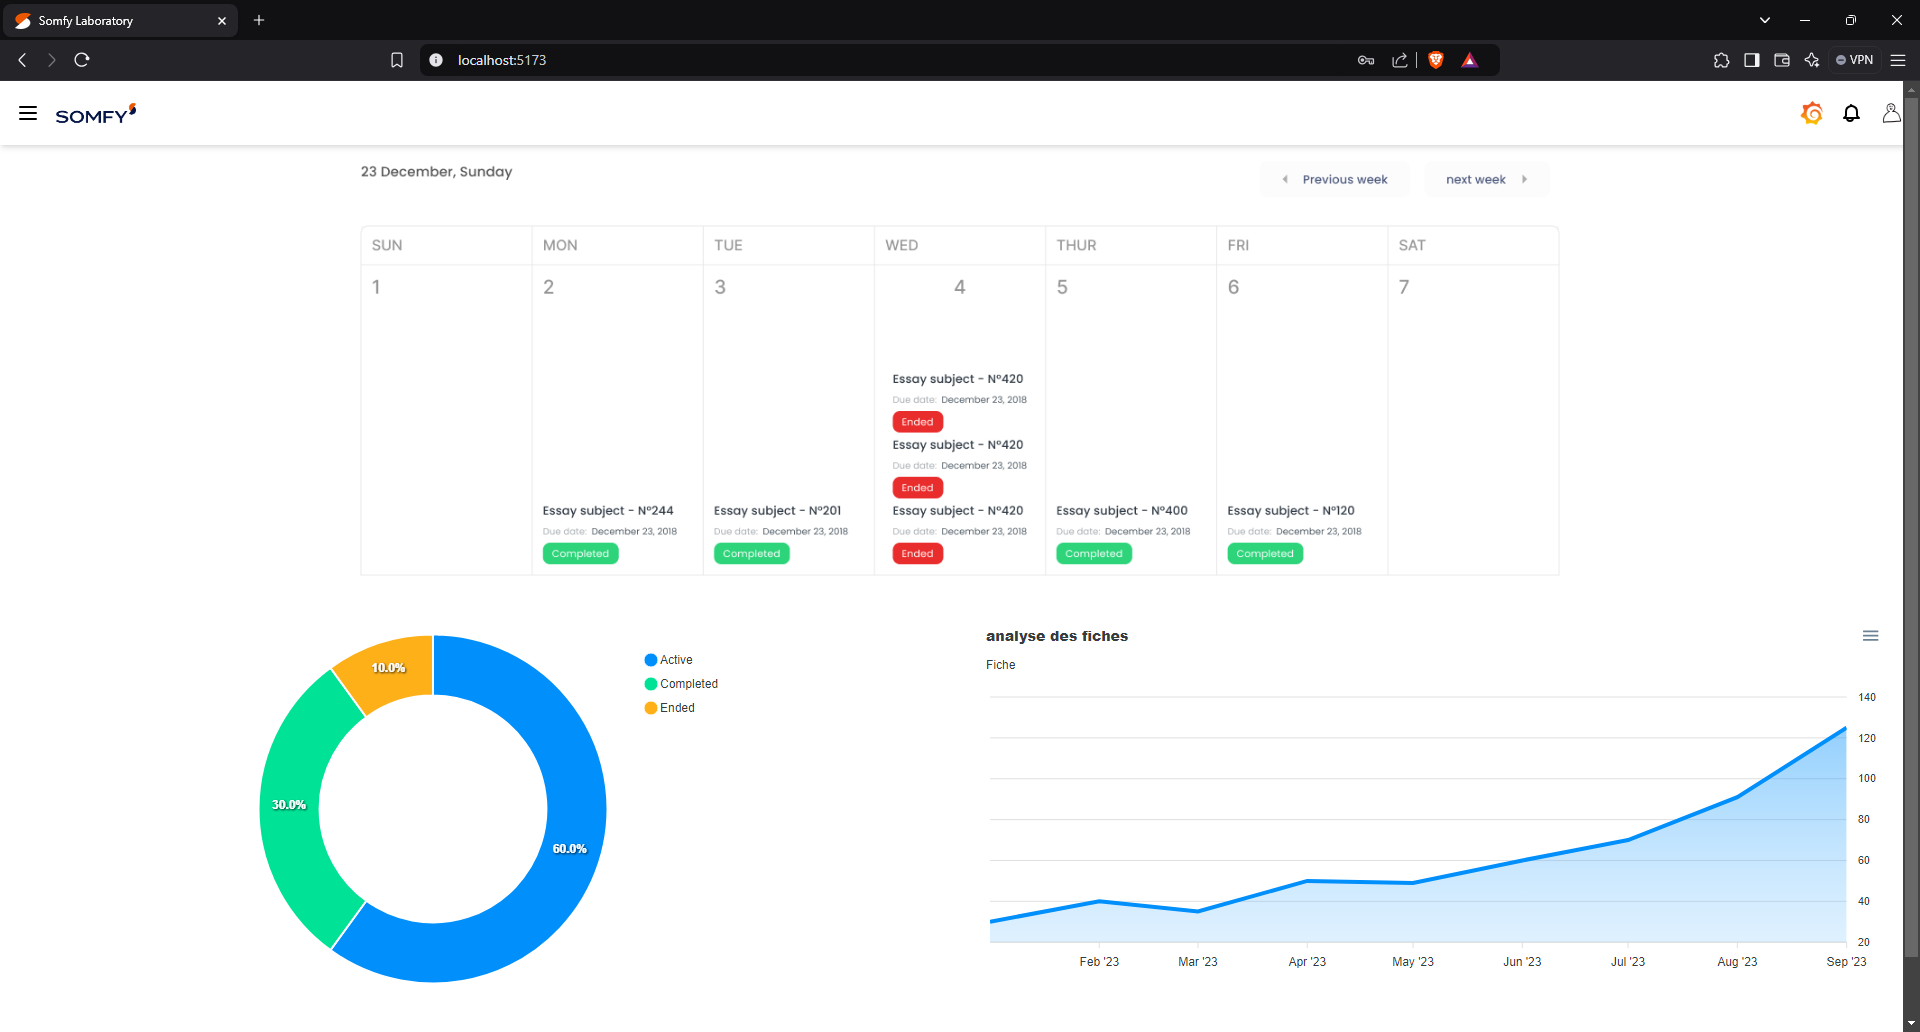
\includegraphics[width=1\textwidth]{chapters/3/img/2.png}
    \caption{cp 242-1 LEAN}
    \label{fig:campus}
\end{figure}


\begin{figure}[H]
    \centering
    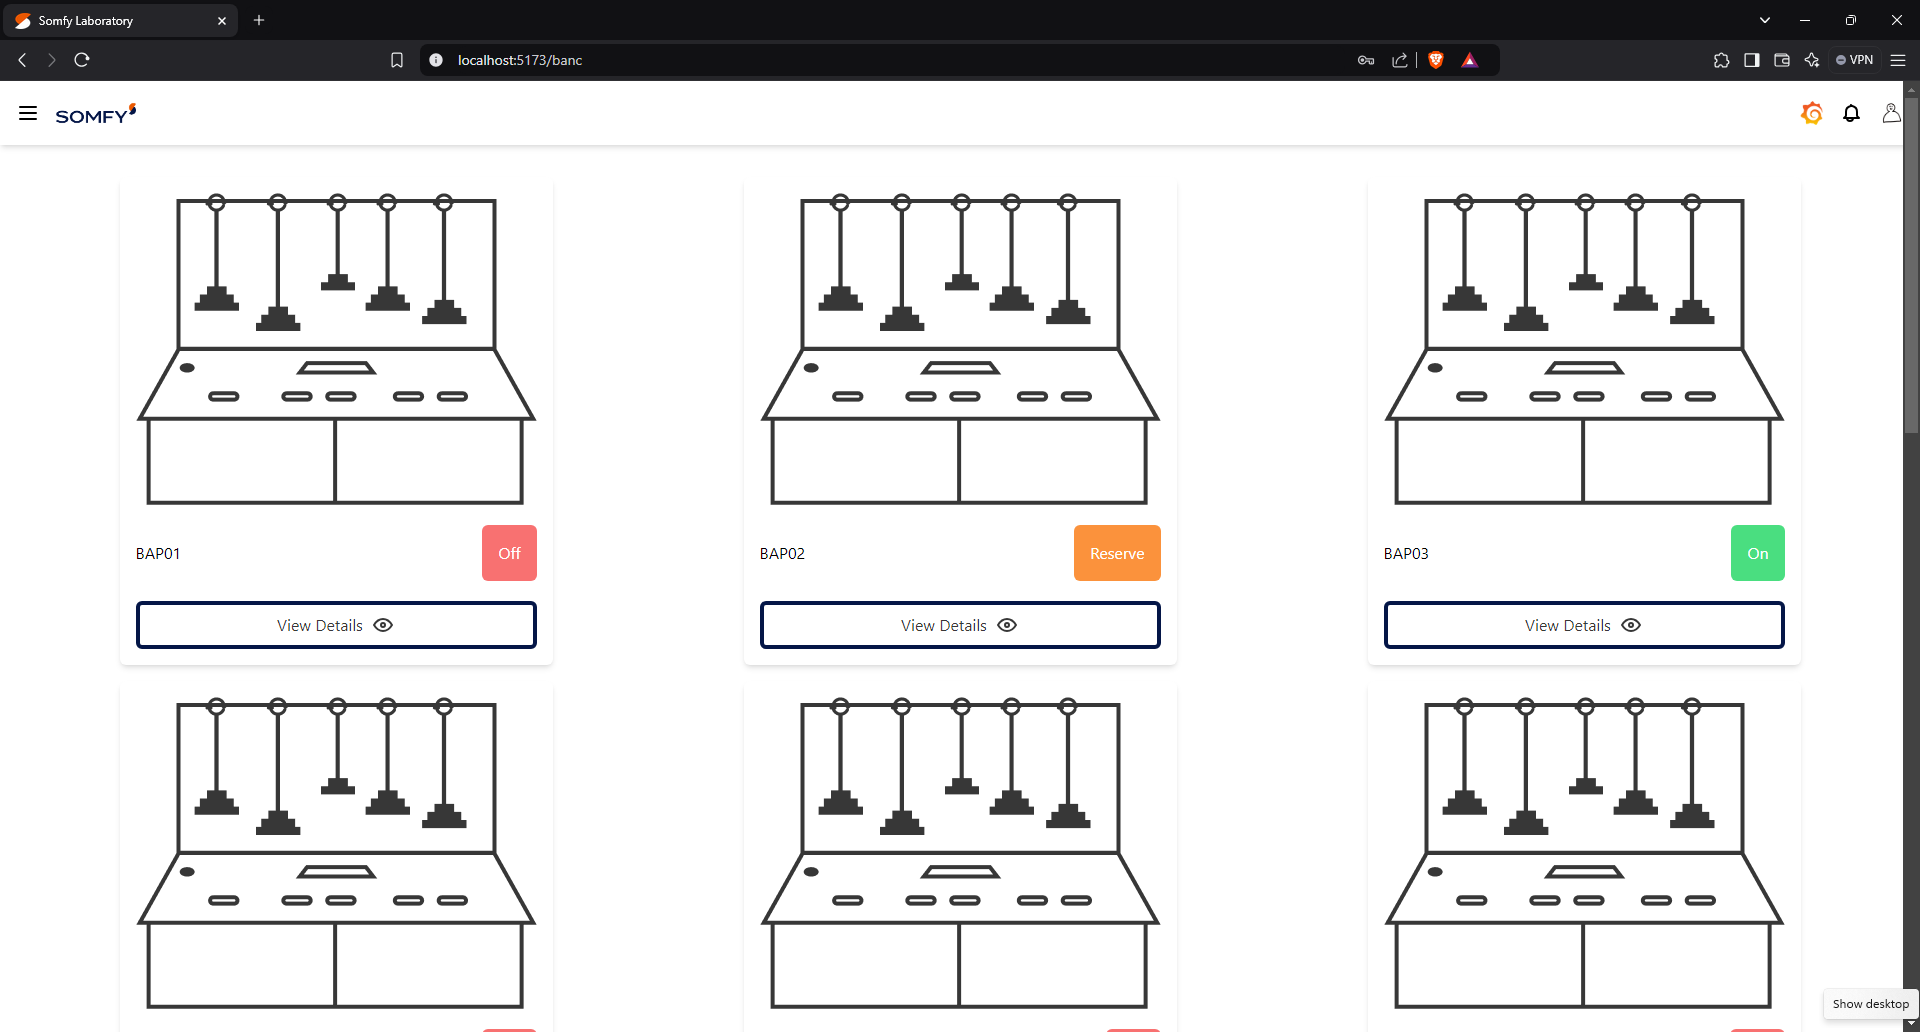
\includegraphics[width=1\textwidth]{chapters/3/img/6.png}
    \caption{cp 242-1 LEAN}
    \label{fig:campus}
\end{figure}










\section{Backend Development}

\subsection{Backend Architecture with ASP.NET Core}
The backend services were developed using ASP.NET Core, which enabled the creation of secure, scalable APIs. This layer handles user authentication, data management, and integration with controllers. Key elements include:
\begin{itemize}
    \item \textbf{API Development}: Exposing endpoints for frontend communication using controllers in ASP.NET.
    \item \textbf{Security Measures}: Implementation of token-based authentication and authorization to protect sensitive data.
    \item \textbf{Data Management}: Interaction with a SQL Server database to store and retrieve information.
\end{itemize}

\subsection{Database Structure}
The database schema was designed to handle the various entities within the LAB.E.S system, including:
\begin{itemize}
    \item \textbf{Equipment Data}: Information about laboratory instruments and their configurations.
    \item \textbf{Test Records}: Data related to different tests performed, linked to equipment and users.
    \item \textbf{User Management}: Storing user profiles, access levels, and activity logs.
\end{itemize}
\begin{figure}[H]
    \centering
    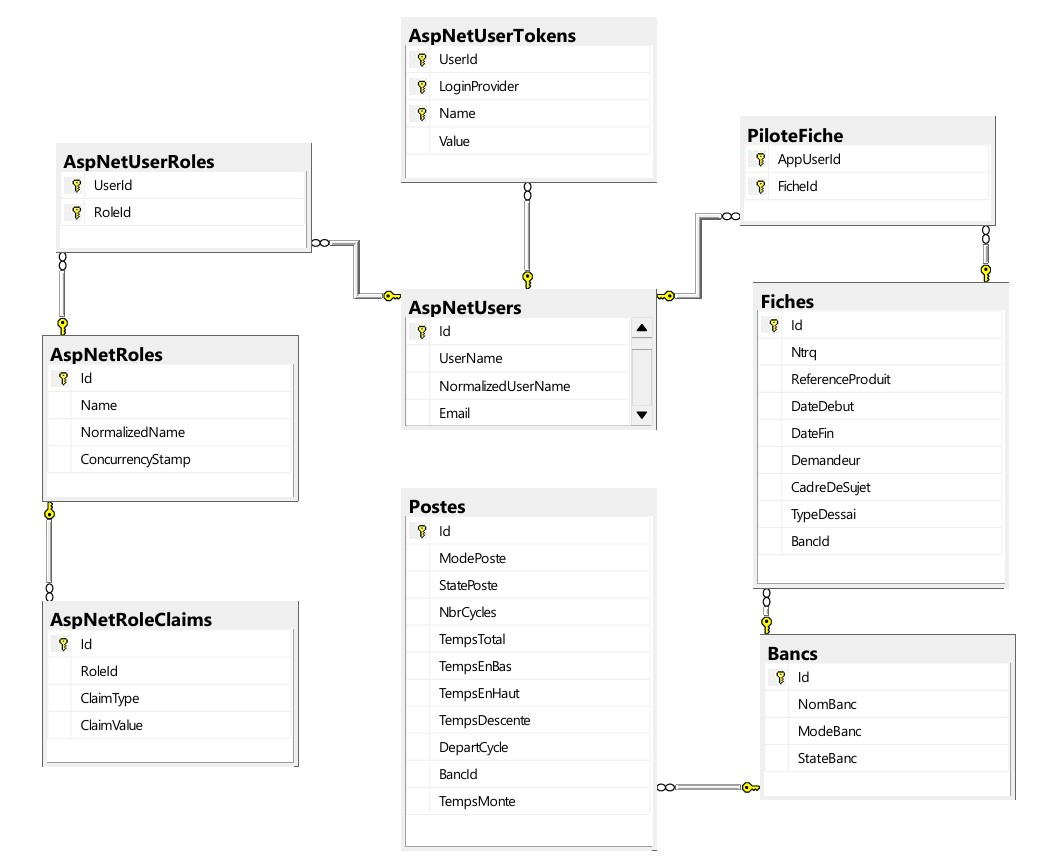
\includegraphics[width=1\textwidth]{chapters/3/img/16.jpg}
    \caption{cp 242-1 LEAN}
    \label{fig:campus}
\end{figure}


\subsection
{Services Déployés dans les iBox}
Pour récupérer les données des automates, plusieurs services ont été déployés sur les iBox :

\subsubsection{Service de Communication :} Gère les échanges de données entre les automates et les systèmes centralisés.
\subsubsection{Service de Stockage :} Assure la collecte et le stockage des données pour une analyse ultérieure.
\subsubsection{Service de Monitoring :} Surveille en temps réel les performances des automates et des flux de données.


\section{Communication and Data Integration}

\subsection{MQTT Protocol}
The MQTT protocol was chosen for its lightweight communication capabilities, particularly suitable for Industrial IoT environments. This enabled real-time updates between the lab equipment and the central system.
\begin{figure}[H]
    \centering
    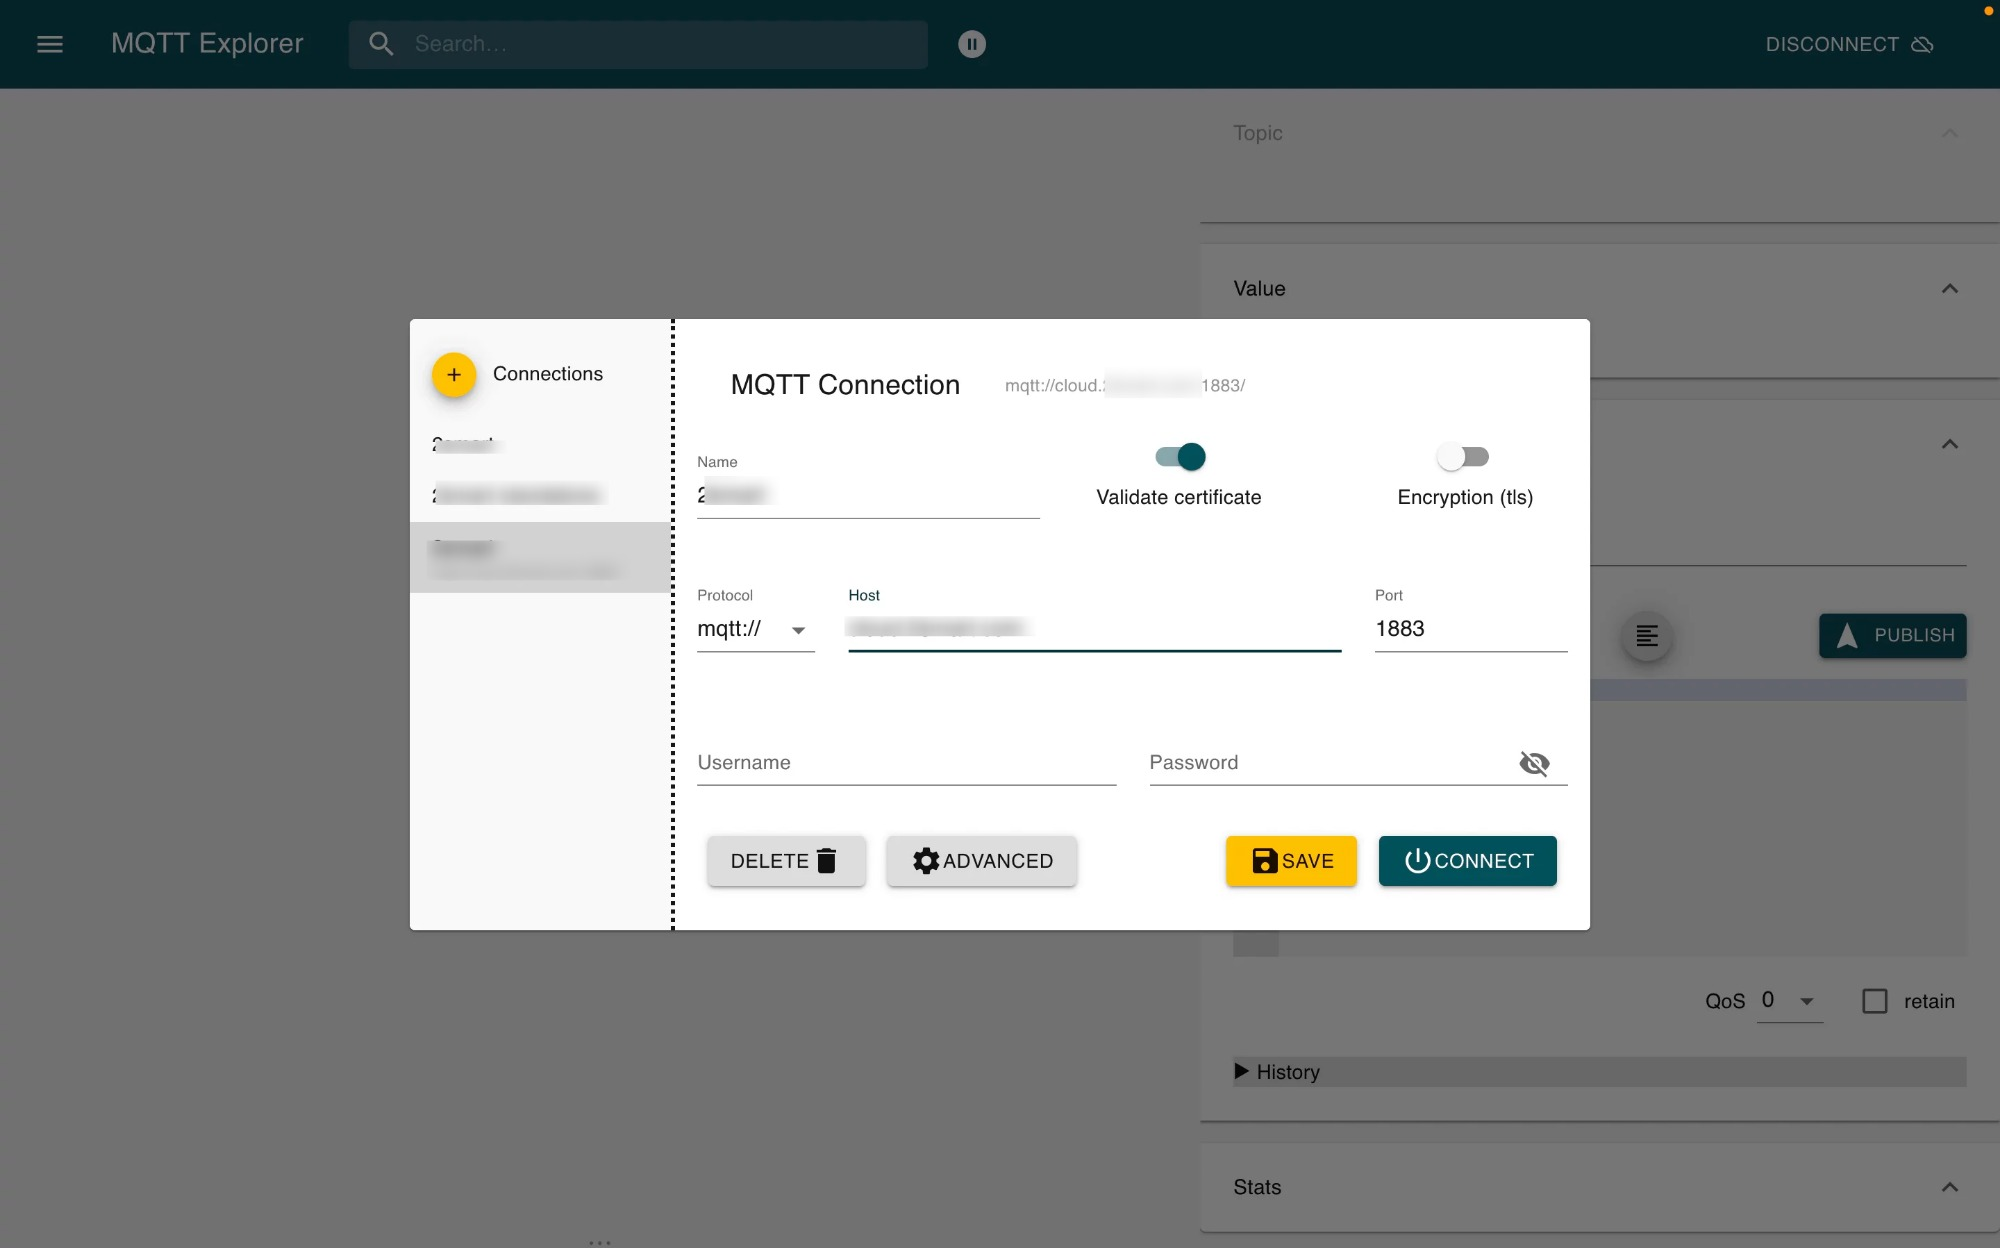
\includegraphics[width=1\textwidth]{chapters/3/img/15.jpg}
    \caption{cp 242-1 LEAN}
    \label{fig:campus}
\end{figure}
\begin{itemize}
    \item \textbf{Data Transmission}: Controllers publish sensor data to the MQTT broker, which is then consumed by backend services for processing.
    \item \textbf{Event-Based Architecture}: The platform reacts to changes instantly, ensuring timely updates and alerts.
\end{itemize}
\begin{figure}[H]
    \centering
    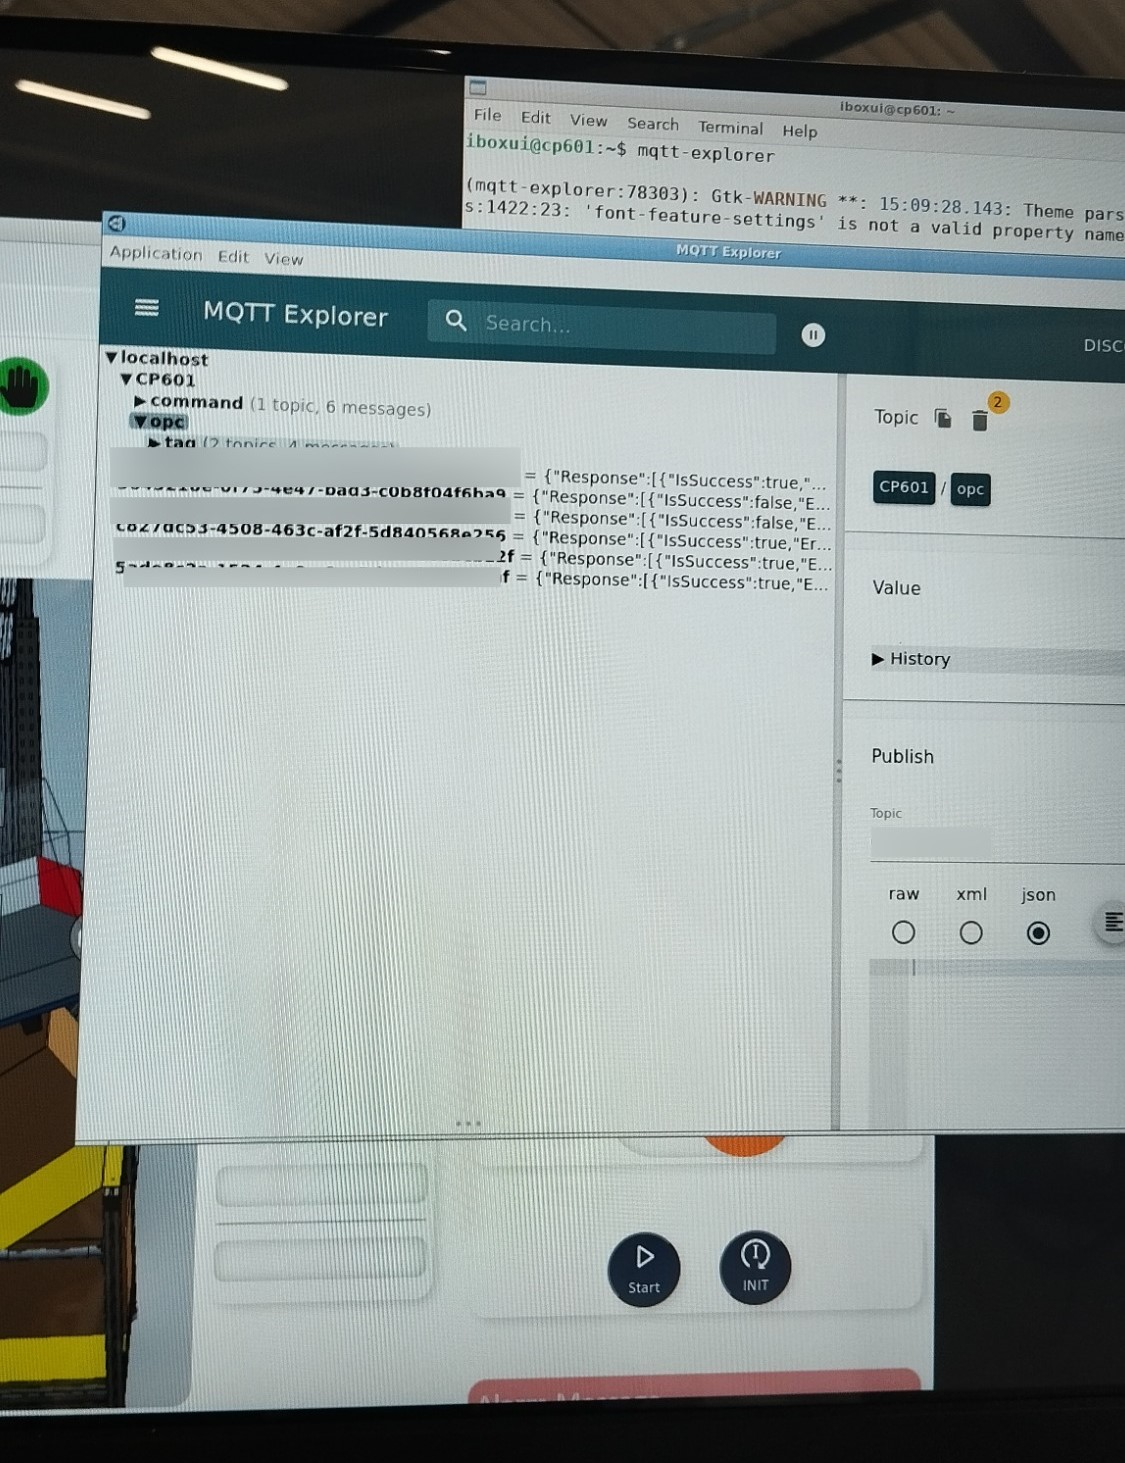
\includegraphics[width=0.6\textwidth]{chapters/3/img/14.jpg}
    \caption{cp 242-1 LEAN}
    \label{fig:campus}
\end{figure}


\subsection{Integration with Industrial Controllers (Step7 Siemens)}
The Siemens Step7 software was used to program controllers that manage laboratory equipment. The controllers were integrated with the LAB.E.S platform via MQTT, enabling automated data collection and control.


\section{IDE Step7 et Programme Automate}
IDE Step7 est l'environnement de développement intégré utilisé pour programmer et configurer les automates S7-300. Cet outil permet de créer des programmes d'automatisation complexes et de configurer les modules de communication.

Programme Automate et Modifications
Pour permettre la récupération des données en temps réel via le CP343-1 Lean, il a été nécessaire d'apporter des modifications au programme des automates. 

Les étapes incluent :
Configuration du CP343-1 Lean : Définition des paramètres réseau et des protocoles de communication.
Mise à Jour du Programme : Adaptation du code existant pour intégrer les nouvelles fonctionnalités de communication.
Tests et Validation : Assurer que les données sont correctement transmises et reçues.
\section{IDEs}

\subsection{Hardware}
\begin{figure}[H]
    \centering
    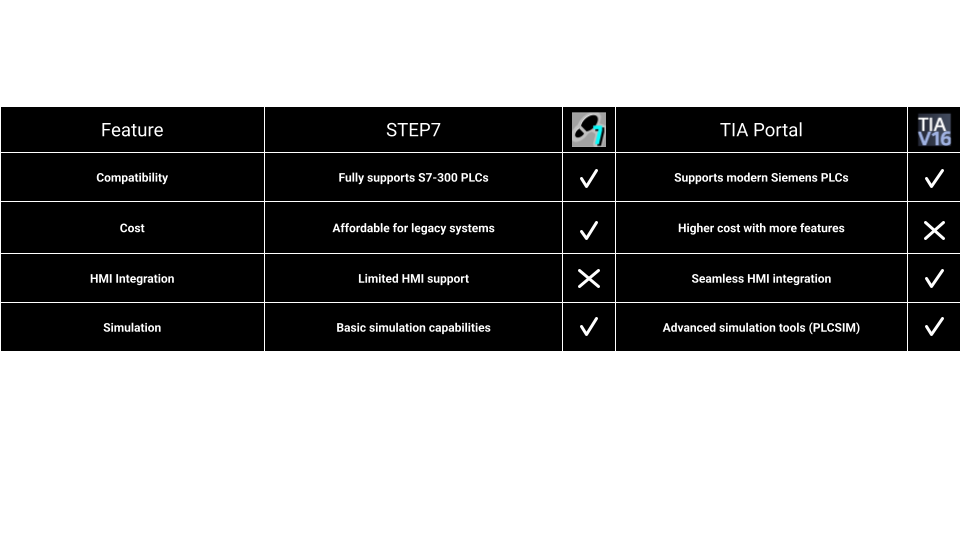
\includegraphics[width=1\textwidth]{chapters/3/img/101.png}
    \caption{cp 242-1 LEAN}
    \label{fig:campus}
\end{figure}

\subsection{UX/UI}
Ensuring real-time data synchronization between controllers and the platform was a challenge due to network latency. This was addressed by optimizing MQTT communication and implementing efficient data caching strategies.

\subsection{Back-end}
Ensuring real-time data synchronization between controllers and the platform was a challenge due to network latency. This was addressed by optimizing MQTT communication and implementing efficient data caching strategies.


\subsection{Fronted}
Ensuring real-time data synchronization between controllers and the platform was a challenge due to network latency. This was addressed by optimizing MQTT communication and implementing efficient data caching strategies.





\chapter{Expérience de Stage}

\section{Introduction}
This chapter details my internship experience working as a developer focusing in test bench infrastructure automation and optimization as part of the LAB.E.S. project. From comprehending user demands to creating technological solutions that were relevant to the laboratory's needs, my position encompassed an extensive list of duties. I was able to improve my technical expertise and skills in project management while adjusting to the demands and limitations of the workplace by actively engaging in team activities.

\clearpage


\section{Poste, Tâches et Responsabilités}
I assumed the position of developer for my LAB.E.S. project, which involved real-time supervision and the implementation and optimization of the test bench infrastructure. Creating automated methods to guarantee dependable testing and effective data collecting procedures was my primary responsibility. Understanding user needs, creating the system architecture, and using contemporary components like the iBox and CP343-1 Lean to enhance communication between various infrastructure components were among my duties.
As a technical team member, I actively participated in a number of departmental tasks. In my free time, I also offered suggestions to the design team to enhance the real-time monitoring platform's user interface. In order to guarantee dependable connections, I also had to supervise the administration of network communications between devices.
Working with the management department to enhance the distribution of laboratory performance and findings was another facet of my involvement.


\section{Formation}
In order to completely comprehend the constraints and difficulties of the current infrastructure, my training started with an examination of the settings and protocols that were already in place. After that, I looked at research and case studies to determine which best practices to use for my project. I gained a thorough understanding of real-time supervisory techniques during this time, as well as the significance of technology decisions for performance improvement.
In a second stage, I attended seminars in the working environment to become acquainted with various industrial devices and received comprehensive training on how to use the iBox. This helped me improve my ability to adjust to real-world work settings and improve my technical abilities for a smooth project integration.

\section{Résultats et Analyse}
Throughout my internship, I encountered a number of difficulties. The biggest obstacle was adjusting to new integrated technologies, including the CP343-1 Lean module, which necessitated plc programming expertise.
Meeting the project's strict budgetary criteria was a further significant challenge. Cost limits and the acquisition of contemporary technology were frequently incompatible, necessitating a rigorous evaluation of priorities and decisions.
Here is a list of the primary difficulties:

1.Adaptability to changes: Testing procedures are slowed down because it frequently takes time to modify test bench setups.
2. Complexity of equipment communication: In the case of unexpected failures or breakdowns, controlling linked equipment became challenging.
3. Lack of specialized training: Not all team members had the specialized training needed to use some outdated equipment, which caused delays in the process.




\section{Conclision}
I was able to get valuable practical skills from my internship, especially in the area of current technology integration and supervision for complex infrastructures. My capacity to handle issues in a professional setting was enhanced by the difficulties I faced, such as controlling communications between components of technology and complying to financial restrictions. In addition to expanding my technical knowledge, this experience has improved my flexibility and critical thinking abilities, which will be extremely useful in my future profession.

% ...
\chapter{Conclusion Générale}

The LAB.E.S project represents a transformative initiative in modernizing laboratory operations by aligning with Industry 4.0 principles. Through the integration of cutting-edge technologies, including IIoT, microservices architecture, and advanced hardware and software solutions, the platform addresses key challenges faced in laboratory management. These efforts contribute to improving efficiency, traceability, and data-driven decision-making.

This report highlights the evolution of the project from its initial conceptualization to its implementation, detailing every critical stage, from identifying user needs and designing user-friendly interfaces to solving real-world challenges such as data synchronization and access restrictions. Moreover, adopting an agile Scrum methodology ensured flexibility and efficient collaboration, while the use of tools like MQTT and ReactJS demonstrates the potential of combining industrial and modern web technologies.

The journey was not without its challenges, such as integrating legacy systems with modern hardware, maintaining budgetary constraints, and resolving communication gaps between devices. However, these obstacles were met with innovative solutions that have laid the foundation for scalable and sustainable operations.

In conclusion, the LAB.E.S project not only achieves its objectives of operational excellence and digital transformation but also serves as a model for future innovations in laboratory management. This experience has provided valuable insights into the importance of technology-driven solutions and their role in industrial progress.

% Bibliographie, utilise bibtex
% NB : biblatex peut également être mis en place mais ce dernier nécessite d'autres packages (ref: la doc)
% ieee ou apalike dépendant des préférences de références.

\end{document}
